\documentclass[11pt,a4paper]{report}

\usepackage{mathtools, amsmath, listings, graphicx, amssymb, nth, cite, multirow, longtable, hyperref, caption}
\usepackage[utf8]{inputenc}
\usepackage[table]{xcolor}

\usepackage{geometry}
\geometry{margin=1in}

\makeatletter

% ------------------ <Convenience Commands> --------------------
\graphicspath{ {figures/} }

\newsavebox\myboxA
\newsavebox\myboxB
\newlength\mylenA

\newcommand*\xoverline[2][0.75]{%
    \sbox{\myboxA}{$\m@th#2$}%
    \setbox\myboxB\null% Phantom box
    \ht\myboxB=\ht\myboxA%
    \dp\myboxB=\dp\myboxA%
    \wd\myboxB=#1\wd\myboxA% Scale phantom
    \sbox\myboxB{$\m@th\overline{\copy\myboxB}$}%  Overlined phantom
    \setlength\mylenA{\the\wd\myboxA}%   calc width diff
    \addtolength\mylenA{-\the\wd\myboxB}%
    \ifdim\wd\myboxB<\wd\myboxA%
       \rlap{\hskip 0.5\mylenA\usebox\myboxB}{\usebox\myboxA}%
    \else
        \hskip -0.5\mylenA\rlap{\usebox\myboxA}{\hskip 0.5\mylenA\usebox\myboxB}%
    \fi}
\makeatother

\hypersetup{colorlinks=true, linkcolor=blue}

\DeclarePairedDelimiter\ceil{\lceil}{\rceil}
\DeclarePairedDelimiter\floor{\lfloor}{\rfloor}

\newcommand{\ts}{\textsuperscript}

% ------------------ </Convenience Commands> --------------------

\begin{document}

% ------------------ Title Page --------------------

\begin{titlepage}
	\centering
	
\includegraphics[width=0.15\textwidth]{brandeis-seal}\par\vspace{1cm}
	{\scshape\LARGE Brandeis University \par}
	\vspace{1cm}
	{\scshape\Large Senior Thesis in Computer Science\par}
	\vspace{1.5cm}
	{\huge\bfseries Graph Matching, Pattern Learning,\par and Protein Domain Modeling \par}
	\vspace{2cm}
	{\Large\itshape Wesley Wei Qian\par}
	\vfill
	supervised by\par
	Prof. \textsc{Pengyu Hong}
	\vfill

	{\large \today\par}
\end{titlepage}

% ------------ Table of Contents ----------------

\tableofcontents

% ----------------- Chapters ----------------------

\chapter*{Acknowledgments}

When I asked Professor Storer to supervise me on a thesis on the graph isomorphism problem, he was hesitant.
He only acquiesced when I persuaded him that my future was secure with a fantastic job, and that my primary objective was the pursuit of questions that were of nothing but personal interest to me.
In many respects, his skepticism proved well founded.

This work has been incredibly challenging, both in that the body of existing work on GI is so large, and in that few visible niches of it exist which are promising and not thoroughly explored.
Over the past year I have poured my time and energy into this project, and have found it unbelievably energizing to do so.
I have been thrilled to find interesting properties in problems surrounding GI, and have had an equal number of frustrations in finding that my results had been previously discovered.
Moreover, it has been illuminating to begin to understand a hidden world of graph theory which had before seemed either trivial or intractably complex.

I would like to thank Professor Storer for the initial bout of skepticism about this project, as it shaped this project and experience for the better.
But I would also like to thank him for the amount of advice and freedom that he has supported me with on this project.
It has kept me on track to focus on my real goal for the semester, which was to learn and grow.
I have learned advanced techniques in GPU calculation, proof techniques in abstract algebra, and gotten the chance to reason with established problems in new and interesting ways.
My skill set has been broadened by this project which has deeply challenged me and always kept me on my toes.

I would like to thank my advisors (Prfs. Storer, Di Lillo and Torrey), the Computer Science department, and my friends and family for all of the different kinds of support and encouragement that have brought me to successful completion of this project.

\chapter*{Abstract}

Given a graph, count the number of closed walks (called cycles) of every length that pass through each vertex in the graph.
Counting the number of cycles gives us a vector which describes a kind of local resonance, a description of the localized area around each vertex within the graph.
This idea is a numerical property, called an invariant, which is highly information dense--able to detect differences between graphs (or vertices) with high probability, but not sufficient to verify that two graphs (or vertices in a single graph) are the same.
It turns out that we can calculate the number of Cycles very quickly, relative to how much information it gives us.

The number of graphs you can create, even over a small number of vertices, is very large.
However, the number is \emph{much} larger if you consider different labelings of the same graph to be distinct.
This difference matters in many contexts, but is made clear through examining standard random graph generators, which treat different labelings of the same graph as if they are different graphs. 
This is not a problem in and of itself (it makes sense in many practical contexts), but it warps theoretic arguments about the runtime of algorithms over `random' graphs, in ways that we can describe through probability, algebraic proof and experimental results.
It turns out that making up our own random graph generators can actually improve upon this state of affairs in a quantifiable way.

\chapter*{An Open Source Project}

An interesting aspect of this thesis has been that I have placed every incremental iteration of my work online, through the git version control system and GitHub.
Every element, from my reading notes, to my mid-semester reports, to my code, results, and datasets: everything has been kept in a central repository, and every change has been committed and logged.
Alongside this choice, I have decided that every line of code I have written is open source and publicly available for use; licensed under the Creative Commons Attribution-ShareAlike 4.0 International License.

There are three reasons to make this thesis as an open source, version controlled work.
\begin{enumerate}
\item{
Research in academia is far too often done in the dark, and only once the conclusion has been drawn and sufficiently polished does the general public get to learn about it. 
This falsely represents scientific inquiry as a lightning bolt, a blinding and stark progression from correct idea to correct idea. 

In reality we all explore ideas that fail, we all have intuitions that turn out to be incorrect.
The reality of research is much more one of lightning's infinitesimally branching electrical charges (with eventual connection and brilliance). Though this report presents a well coordinated and rehearse set of conclusions, this is not a reflection of all of the work that was done. The GitHub source provides the other pieces of this puzzle.
}
\item{I work on a personal laptop, a school desktop, and occasionally a public workstation. Transferring data (of all sorts) between these computers is tiresome and error prone without a VCS.}
\item{Everyone does better work when they know that their work could be observed.}
\end{enumerate}

The work is available \href{http://www.github.com/gbdubs/thesis}{on my personal github page}, and will be there for the foreseeable future.

\chapter{Graph Matching}
\label{chap: graphmatching}

\section{Introduction}

In order to extract the common pattern from graphs, we need to first compare two graphs and match\footnotemark the relevant part together to better summarize them. However, since the largest common subgraph problem is NP-complete, the graph matching problem we are dealing with is also NP-complete (even though you can argue it's NP-hard in some other definition). Therefore, we must look for good suboptimal solutions via approximation.
\footnotetext{The graph matching here is different than the "matching" problem in graph theory where the \emph{matching} is a set of pairwise non-adjacent edge.}\\

There are two main approaches for graph matching. One approach involves the construction of a state-space that can be searched via some brach and bound methods. While some heuristic rule can help us reduce the complexity from exponential to polynomial, the polynomial complexity would still have a high complexity. The second approach employs nonlinear optimization methods like relaxation labeling, which do not search based on the state-space and generally have a much lower computational complexity.\\

In the realm of nonlinear optimization methods and similar to relaxation labeling, here we described a graduated assigned approach developed by Gold and Rangarajan in 1996 and the improvement we made on the algorithm in order deal with larger graphs we encounter today 20 years later.

\section{Syntax and Definition}

Here we use a attributed relational graph (ARG) to represent our spatial pattern. An ARG, $G$, is a \emph{directional} graph with labels on its nodes ($\overrightarrow{N_{a}}$ is the label for the $a$th node in the graph) and edges ($\overrightarrow{E_{ab}}$ is the label for the edge from the $a$th node to the $b$th node). \\

Since two graphs might only match partially by their subgraph or might not have match at all, Gold and Rangarajan add a null node, $\phi$, in each ARG.\\

We then can define the node compatibility function($c_N$) and the edge compatibility function($c_E$) to calculate the compatibility, $C$, between the nodes and edges between two ARGs, $G$ and $G'$. Here, $C_{ai}$ is the compatibility between node $\overrightarrow{N_{a}}$ in $G$ and node $\overrightarrow{N_{i}}$ in $G'$, while $C_{abij}$ is the compatibility between edge $\overrightarrow{E_{ab}}$ in $G$ and $\overrightarrow{E_{ij}}$ in $G'$.\\

The match result is defined as a matrix $M$ where $M_{ai}$ is the probability matching the $a$th node in $G$ to the $i$th node in $G'$.

\section{Problem Definition}

We defined the problem of ARG matching in the following manner. Given two ARG, $G$ and $G'$, we want to find the match matrix $M$ such that the following objective function is minimized:

\begin{equation}\label{eq:energy}
E(M)=-\frac{1}{2}\sum_{a=1}^{G}\sum_{i=1}^{G'}\sum_{b=1}^{G}\sum_{j=1}^{G'}M_{ai}M_{bj}C_{abij}-\alpha\sum_{a=1}^{G}\sum_{i=1}^{G'}M_{ai}C_{ai}
\end{equation}
subject to a two way constraints: $\forall a\ne\phi$, $\sum_{i=1}^{G'}M_{ai}=1$ and $\forall i\ne\phi$, $\sum_{i=1}^GM_{ai}=1$:

\begin{figure}[h]
	\centering
	\captionsetup{justification=centering}
	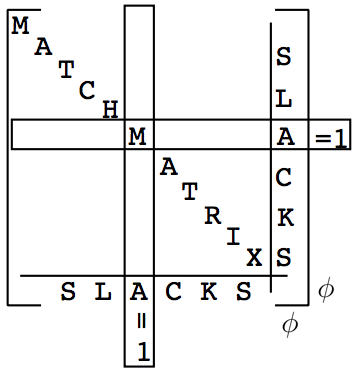
\includegraphics[width=0.25\textwidth]{figs/two_way_constraints.png}
	\caption[Caption for LOF]{\emph{Both rows and columns should sum up to 1 except the row and column involving $\phi$ nodes, which are considered the slack row and slack column.}}
	\label{fig:two_way_constraints}
\end{figure}

\section{Graph Matching by Gold and Rangarajan}

In Gold and Rangarajan's original algorithm, they solve the problem using a graduated assignment method where the two-way constraints are satisfied by normalizing rows and columns iteratively for many rounds (Sinkhorn 1963) and their compatibilities are defined as:
\begin{align} 
& C_{ai}  = \begin{cases}0 & a=\phi \bigcup i=\phi \\c_N(\overrightarrow{N_{a}},\overrightarrow{N_{i}}) & otherwise\end{cases}\\
& C_{abij} = \begin{cases}0 & a=\phi \bigcup b=\phi \bigcup i=\phi \bigcup j=\phi \\c_E(\overrightarrow{E_{ab}},\overrightarrow{E_{ij}}) & otherwise\end{cases} 
\end{align}\\

To expand on their graduated assignment method, we will first need to convert our objective function to an assignment problem. They way we do it is through Taylor series approximation, where given an initial $M^0$, we would have:
\begin{align}
E(M) = & -\frac{1}{2}\sum_{a=1}^{G}\sum_{i=1}^{G'}\sum_{b=1}^{G}\sum_{j=1}^{G'}M_{ai}M_{bj}C_{abij}-\alpha\sum_{a=1}^{G}\sum_{i=1}^{G'}M_{ai}C_{ai}\nonumber\\
= & -\frac{1}{2}\sum_{a=1}^{G}\sum_{i=1}^{G'}\sum_{b=1}^{G}\sum_{j=1}^{G'}M_{ai}^{0}M_{bj}^{0}C_{abij}-\alpha\sum_{a=1}^{G}\sum_{i=1}^{G'}M_{ai}^{0}C_{ai} - Q_{ai}(M_{ai}-M_{ai}^{0})
\end{align}
where
\begin{equation} 
Q_{ai}=-\frac{\partial E}{\partial M_{ai}}\bigg\rvert_{M=M_0}=+\sum_{b=1}^{G}\sum_{j=1}^{G'}M_{bj}^{0}C_{abij}+\alpha C_{ai}
\end{equation}\\

Therefore, minimizing our objective function $E$ based on our Taylor series expansion is equivalent to maximizing 
\begin{equation}
+\sum_{a=1}^{G}\sum_{i=1}^{G'}Q_{ai}M_{ai}
\end{equation}
which is an assignment problem!\\

Therefore, we can run the following algorithm for the graduated assignment:\\
\\
\textbf{Initialize} $\beta$ to $\beta_{0}$, $M_{ai}$ to a random sample from $U(0,1)$\\
\textbf{Begin $A$:} (Do $A$ until $\beta \geq \beta_{f}$)\\
\indent \textbf{Begin $B$:} (Do $B$ until $M$ converges or \# of iterations $>I_0$)\\
\indent $Q_{ai} \leftarrow \sum_{b=1}^{G}\sum_{j=1}^{G'}M_{bj}^{0}C_{abij}+\alpha C_{ai}$\\
\indent $M_{ai}^{0} \leftarrow exp(\beta Q_{qi})$\\
\indent \indent \textbf{Begin $C$:} (Do $C$ until $M$ converges or \# of iterations $>I_1$)\\
\indent \indent  Update $M$ by normalizing across all rows:\\
\indent \indent  $M_{ai}^{1}=\frac{M_{ai}^{0}}{\sum_{i=1}^{G'}M_{ai}^{0}}$ for all $a\neq\phi$\\
\indent \indent  Update $M$ by normalizing across all columns:\\
\indent \indent  $M_{ai}^{0}=\frac{M_{ai}^{1}}{\sum_{a=1}^{G}M_{ai}^{1}}$ for all $i\neq\phi$\\
\indent \indent \textbf{End $C$}\\
\indent \textbf{End $B$}\\
$\beta\leftarrow\beta_{r}\beta$\\
\textbf{End $A$}\\
\textbf{Perform Clean-up Heuristic}\\

Variable and constant definitions can be found as:
\begin{figure}[h]
	\centering
	\captionsetup{justification=centering}
	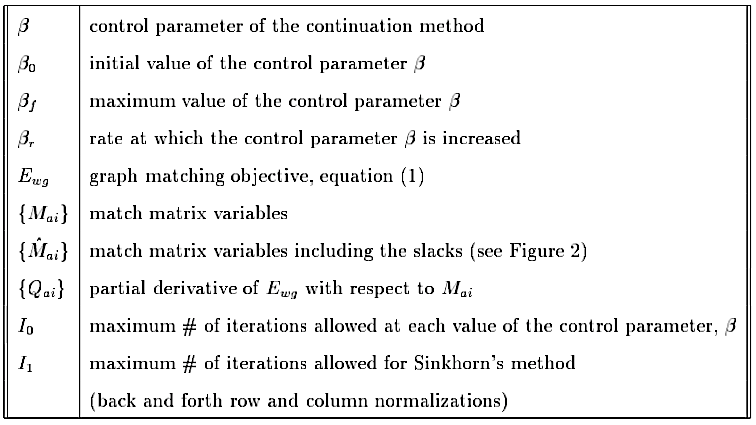
\includegraphics[width=0.95\textwidth]{figs/algorithm_variable.png}
\end{figure}

\section{Implementation Detail}

\subsection{Compatibility}
\label{ssec:compatibility}

To calculate the compatibility, we assume the label/feature follows a Gaussian probability distribution function so that the compatibility function $c_N$ and $c_G$ is defined as:
\begin{equation} 
c_N( \overrightarrow{a}, \overrightarrow{b} )=c_E( \overrightarrow{a}, \overrightarrow{b})=\frac{exp(-\frac{1}{2}(\overrightarrow{a}-\overrightarrow{b})^{T}\Sigma^{-1}(\overrightarrow{a}-\overrightarrow{b})}{(2\pi)^{\zeta/2}|\Sigma|^{1/2}}
\end{equation}
where $\delta$ is the covariance matrix and $\zeta$ is the dimension of $\overrightarrow{a}$ and $\overrightarrow{b}$. Since we assume feature independence, the covariance matrix $\delta$ is the identity matrix, which essentially will give us:
\begin{equation} 
c_N( \overrightarrow{a}, \overrightarrow{b} )=c_E( \overrightarrow{a}, \overrightarrow{b})=\frac{exp(-\frac{1}{2}(\overrightarrow{a}-\overrightarrow{b})^{T}(\overrightarrow{a}-\overrightarrow{b})}{(2\pi)^{\zeta/2}}
\end{equation}

\subsection{Parallel Computing and Caching}

The majority of the computation complexity in the algorithm is in computing the compatibility, especially the edge compatibility.\\

Since the compatibility function defined can be computer independently, one way we could speed up the algorithm is calculating the compatibility in parallel fashion.\\

Another way we could improve the computation time would be through caching, where we can pre compute a node and edge compatibility matrix, as the label is never updated. However, the edge compatibility matrix can be very large and takes a lot of memory to cache, so you might also want to use data structure like \emph{sparse matrix} since the connection matrix (representing edge) is likely to be sparse as well.

\subsection{Heuristic}

In our implementation, we use a very simple heuristic to clean up the match matrix $M$ from a \emph{softassign} matrix to a matrix only with $0$ and $1$. We simply set the largest value (at index $j$) for each row $i$ to 1 and other value to 0. After setting $M_{ij}$ to 1, we also set the entire $j$ column to 0 in order to satisfy the two-way constraints.\\

If you want to be more fancy about this, you can also convert this heuristic problem to a maximum spanning tree problem to make sure all the $M_{ij}$ that you set to 1 have the largest sum.

\subsection{Converge Condition}

In our implementation, we compare the previous match matrix $M^{(0)}$ and the current match matrix $M^{(1)}$, and conclude the matrix converge if the difference is less than some threshold $\iota$:

\begin{equation} 
\sum_{a=1}^{G}\sum_{i=1}^{G'}|M_{ai}^{(0)}-M_{ai}^{(1)}|<\iota
\end{equation}

\subsection{Run Time}
\label{ssec:graphmatchingruntime}

The algorithm takes $\sim15s$ to complete when matching two graphs with $\sim30$ nodes. However, you can certainly adjust the parameter like $I$ and $\beta$ to achieve faster run time.

\section{Testing the Algorithm}
\label{sec:graphmatchingtest}

To test the algorithm, we first set a noise level $\epsilon \in [0,1]$. Then we generate a pattern with $n$ nodes and embed this pattern to $2$ randomly generated graphs, $G$ and $G'$, with $n$ to $n*(1+\epsilon)$ nodes. Once we embed the pattern in these two random graphs, we shuffle the index for each node and add some noise to the node and edge labels:

\begin{equation} 
\overrightarrow{N_{a}} \leftarrow \overrightarrow{N_{a}}  + \chi*\overline{N} \text{ where } \chi \in [0,\epsilon]
\end{equation}
\begin{equation} 
\overrightarrow{E_{ab}} \leftarrow \overrightarrow{E_{ab}}  + \chi*\overline{E} \text{ where } \chi \in [0,\epsilon]
\end{equation}\\

We then run the matching algorithm $match(G,G')$ and get a match matrix $M$. We ignore the match with the null node $\phi$, and calculate the total number of correct match $m$, and the total number of match observed $l$ from the match matrix $M$. Then we can evaluate the performance by $precision$, $recall$ and $F_1 score$:
\begin{align} 
& precision = \frac{m}{l}\\
& recall = \frac{m}{n}\\
& F_1 =2*\frac{precision*recall}{precision+recall}
\end{align}

\section{Improvement and Modification}

While the original algorithm works well with small graphs with 20 to 30 nodes, we run into some problems while matching larger graphs with 50 to 100 nodes and therefore make some improvement to Gold and Rangarajan's original algorithm.

\subsection{Local Minima}

The first problem we encounter is local minima. In this case, the algorithm will generate correct and even perfect match for majority of the test cases. However, for some of the test case, the match result is entirely wrong, which indicates that the graduated assignment process stuck in some local minima.\\

In the original algorithm, if we initialized $M_0$ in the wrong places, the assignment process can easily get stuck in sub-optimal match (local minima). While adjusting $\beta$ and $\beta_r$ can mediate the problem, it does not work well in larger graphs since there are more sub-optimal match. Therefore, we introduce a stochastic process in the algorithm:

\begin{figure}[h]
	\centering
	\captionsetup{justification=centering}
	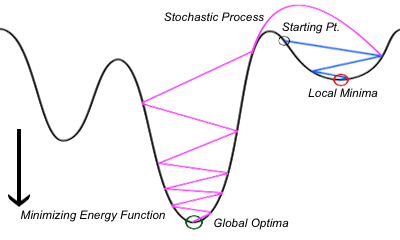
\includegraphics[width=0.46\textwidth]{figs/stochastic.png}
	\caption[Caption for LOF]{\emph{The intuition behind introducing the stochastic process.}}
	\label{fig:stochastic}
\end{figure}

In the stochastic process, we essentially add some small noise to the match matrix at the beginning of step \textbf{$B$}:
\begin{equation} 
M_{ai}^{0} \leftarrow M_{ai}^{0} + \frac{\tau * U(-1,1)}{|G|}
\end{equation}
where $\tau$ is the stochastic/noise level, $|G|$ is the number of node in $G$, and $U(-1,1)$ is a random sample from a uniform distribution between $-1$ and $+1$.\\

Therefore, the updated algorithm becomes:\\
\\
\textbf{Initialize} $\beta$ to $\beta_{0}$, $M_{ai}$ to a random sample from $U(0,1)$\\
\textbf{Begin $A$:} (Do $A$ until $\beta \geq \beta_{f}$)\\
\indent \textbf{Begin $B$:} (Do $B$ until $M$ converges or \# of iterations $>I_0$)\\
\indent \textcolor{red}{$M_{ai}^{0} \leftarrow M_{ai}^{0} + \frac{\tau * U(-1,1)}{|G|}$}\\
\indent $Q_{ai} \leftarrow \sum_{b=1}^{G}\sum_{j=1}^{G'}M_{bj}^{0}C_{abij}+\alpha C_{ai}$\\
\indent $M_{ai}^{0} \leftarrow exp(\beta Q_{qi})$\\
\indent \indent \textbf{Begin $C$:} (Do $C$ until $M$ converges or \# of iterations $>I_1$)\\
\indent \indent  Update $M$ by normalizing across all rows:\\
\indent \indent  $M_{ai}^{1}=\frac{M_{ai}^{0}}{\sum_{i=1}^{G'}M_{ai}^{0}}$ for all $a\neq\phi$\\
\indent \indent  Update $M$ by normalizing across all columns:\\
\indent \indent  $M_{ai}^{0}=\frac{M_{ai}^{1}}{\sum_{a=1}^{G}M_{ai}^{1}}$ for all $i\neq\phi$\\
\indent \indent \textbf{End $C$}\\
\indent \textbf{End $B$}\\
$\beta\leftarrow\beta_{r}\beta$\\
\textbf{End $A$}\\
\textbf{Perform Clean-up Heuristic}\\

Once we incorporate the stochastic process to the algorithm, we gain a significant improvement in $F_1$ score and there is very little chance the match result is entirely wrong:

\begin{figure}[h]
	\centering
	\captionsetup{justification=centering}
	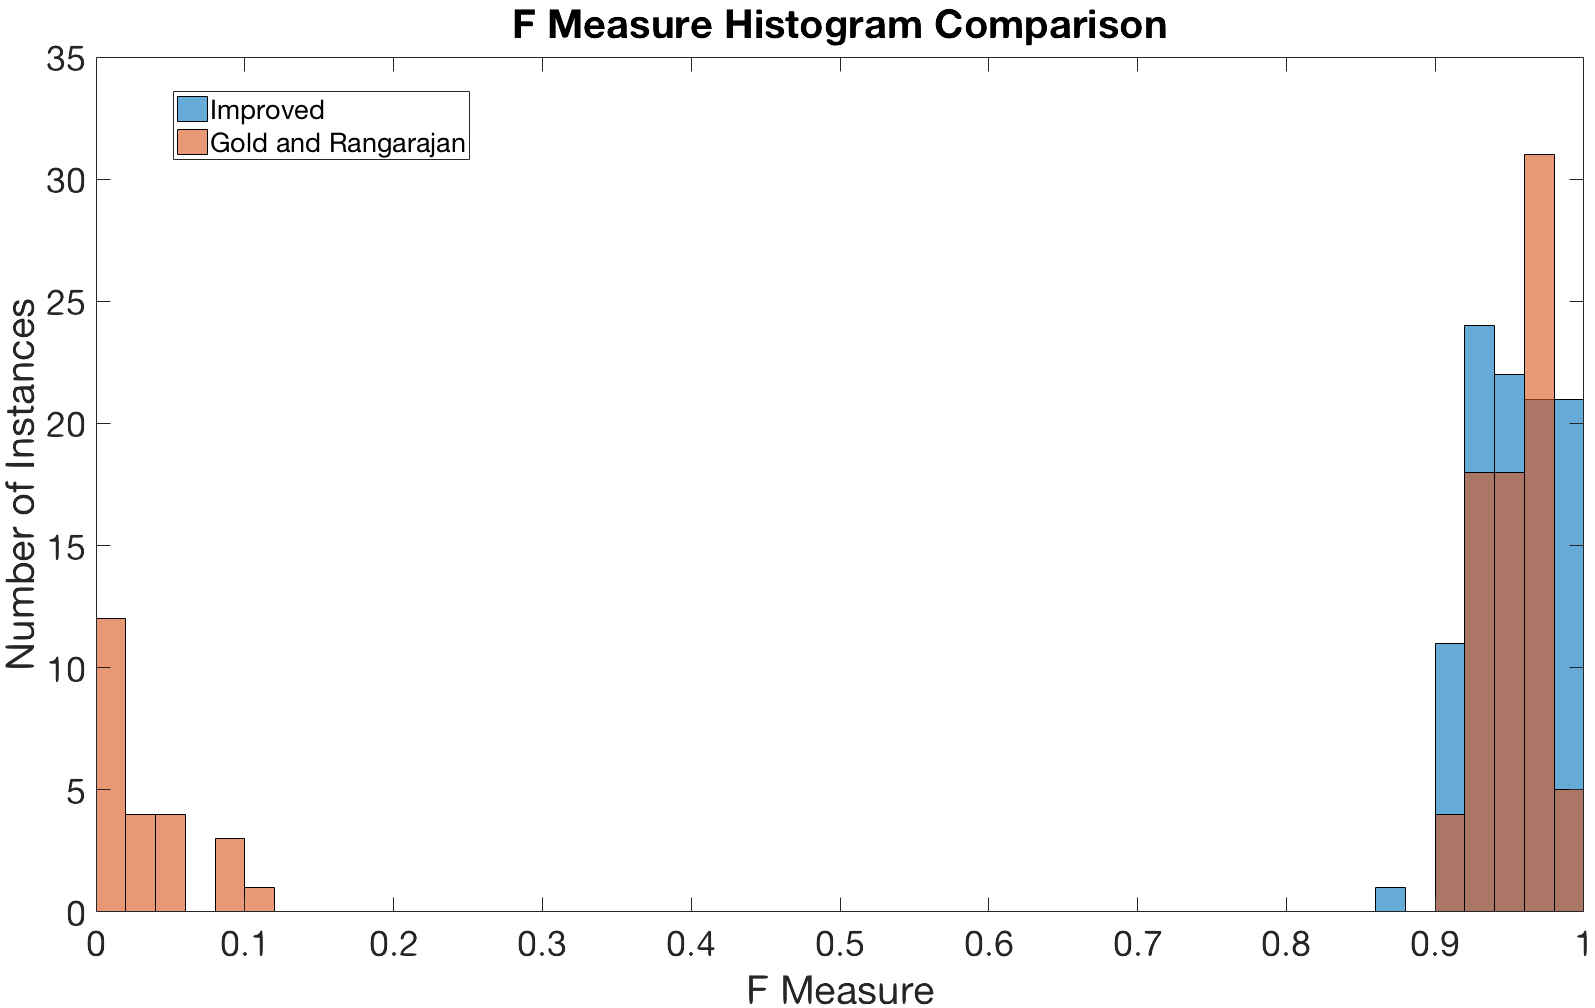
\includegraphics[width=0.85\textwidth]{figs/s_improved.png}
	\caption[Caption for LOF]{\emph{$F_1$ score distribution histogram for the original algorithm (orange) and the improved algorithm with stochastic process (blue).}}
	\label{fig:stochastic}
\end{figure}

\subsection{High Recall + Low Precision}
\label{ssec:nullnode}

The other challenge we encounter is that even though we get high recall rate in a test, we also get low precision rate, which means the algorithm can generate correct match but also force many of the background nodes (i.e. nodes outside of the pattern) matching  to each other.\\

The first explanation came across our mind would be the two test graphs we generated can share pattern outside the embedded one. However, after careful examination, this is proven not the case.\\

Therefore, we examed how Gold and Rangarajan's original algorithm matches background nodes in $G$ to the null node $\phi$ in $G'$. We realized that since the original algorithm define the compatibility function so that any compatibility related to the $\phi$ node will be set to 0. Therefore, the algorithm does not \emph{actively} match background nodes to  $\phi$ node, but \emph{hope} that the background noise does not attract to one specific node, and end up matching with the $\phi$ node.\\

To handle this problem gracefully, we essentially want to create a fully connected null node network that can match to any of the background pattern. Therefore, we rewrite the compatibility function as:

\begin{align} 
& C_{ai}  = \begin{cases}
0 & a,i=\phi \\
c_N(\overrightarrow{N_{a}},\overrightarrow{N_{i}}) & a, i\neq\phi \\
p \text{ percentile of }[C_{1i}, C_{2i},...C_{|G|-1i}] & a=\phi\\
p \text{ percentile of }[C_{a1}, C_{a2},...C_{a|G'|-1}] & i=\phi
\end{cases}\\
& C_{abij} = \begin{cases}
c_E(\overrightarrow{E_{ab}},\overrightarrow{E_{ij}})  & a,b,i,j\neq\phi \\
p \text{ percentile of }\{C_{abij}|a,b,i,j\neq\phi\} & a,b\neq\phi \bigcap i,j=\phi\\
p \text{ percentile of }\{C_{abij}|a,b,i,j\neq\phi\} & a,b=\phi \bigcap i,j\neq\phi\\
0 & otherwise\\
\end{cases}
\end{align}
where $p$ is a percentile we can adjust so that set to 100 to give null node/edge the maximum compatibility every seen while set to 0 to give the minimum compatibility. You can adjust the $p$ to balance the recall and precision rate since higher percentile will encourage nodes match to null node result in low recall but high precision while lower percentile will allow background nodes match together result in high recall but low precision.\\

While this is a lot to unpack, the updated compatibility function essentially create a self-linked edge for null node $\overrightarrow{E_{\phi\phi}}$ and give definition for the compatibility of null node to other real node and self-linked null edge to other edge linking two real nodes. Since we don't normalized the slack row and column (match result for null node), this is equivalent to create a fully connected null node network:

\begin{figure}[h]
	\centering
	\captionsetup{justification=centering}
	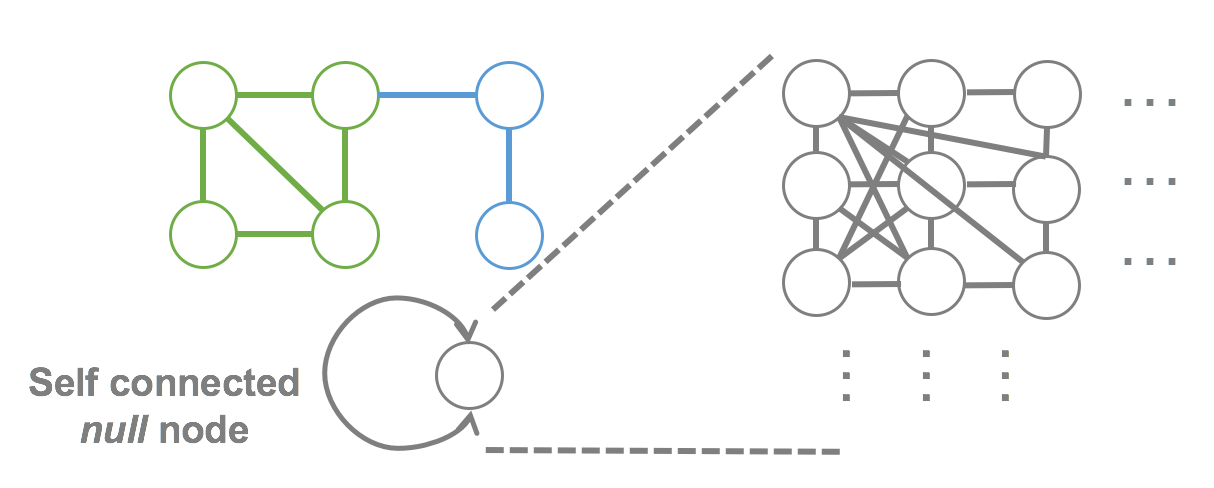
\includegraphics[width=0.46\textwidth]{figs/null_node_network.png}
	\caption[Caption for LOF]{\emph{The self linked/connected null node $\phi$ (grey) can be treated as a fully connected null node that can be matched to any pattern including background nodes. }}
	\label{fig:stochastic}
\end{figure}

After modified the compatibility function in the original algorithm, we are able to generate match result with both high recall and high precision. For instance, two graph with backgrounds nodes at the beginning and the end (in terms of their index) are not forced to match to each other (left) and end up match to the null node/the slack column/row in the end (right):
\begin{figure}[h]
	\centering
	\captionsetup{justification=centering}
	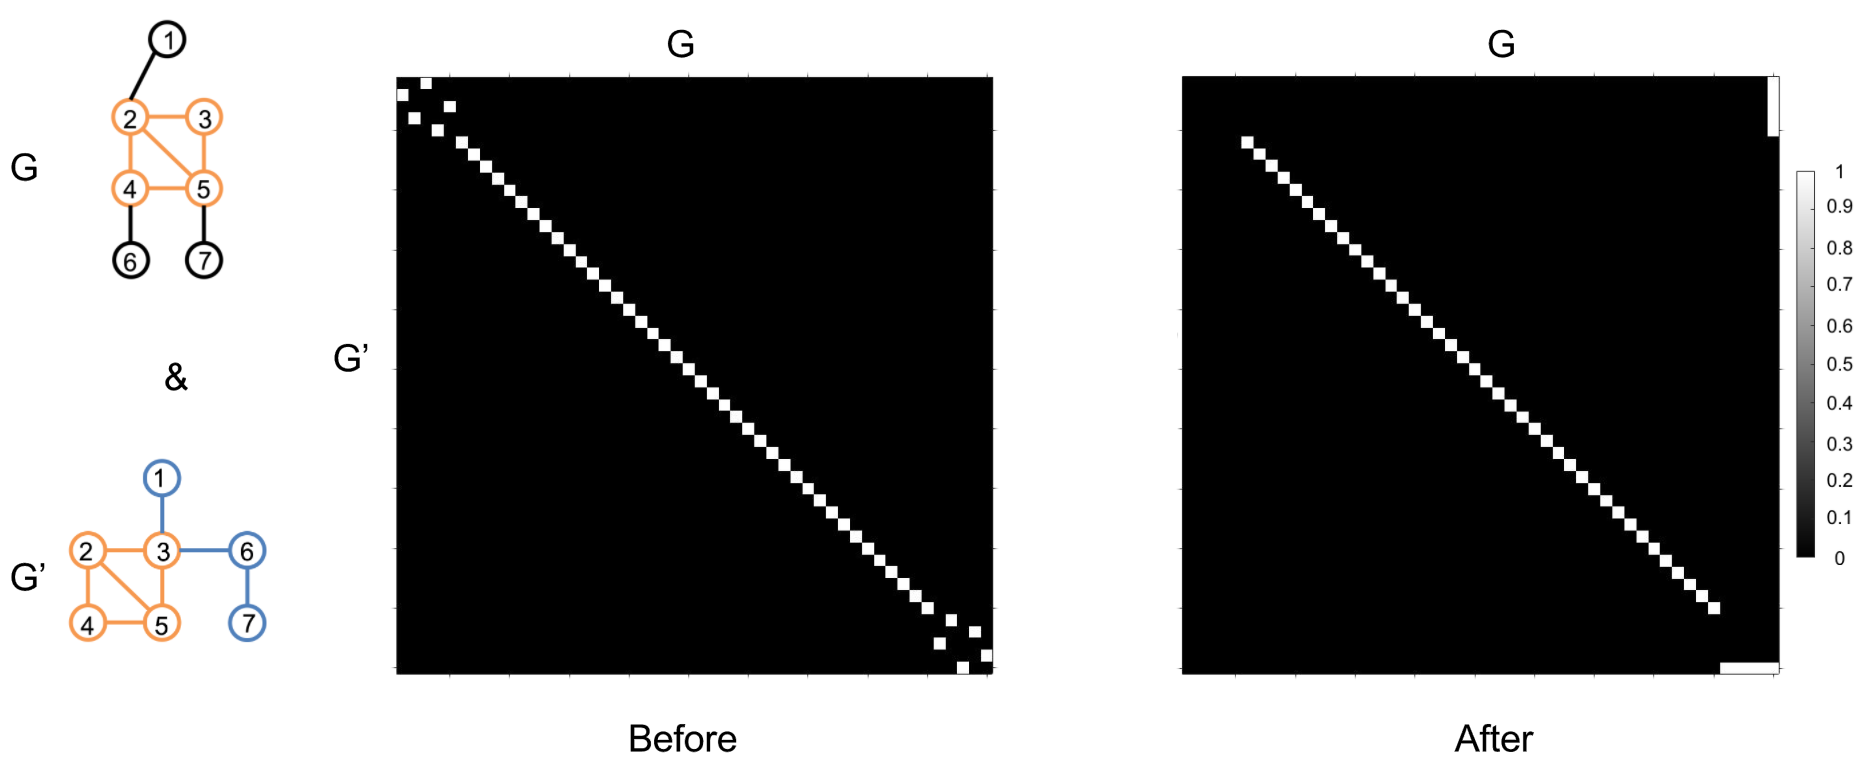
\includegraphics[width=0.8\textwidth]{figs/null_node_improve.png}
	\caption[Caption for LOF]{\emph{This is a visualization of the match matrixes produced by the original algorithm by Gold and Rangarajan (left) and the modified version (right).}}
	\label{fig:stochastic}
\end{figure}

\section{Conclusion}


In this chapter we introduced a graph matching algorithm that we improved and used to match the common sub-graph of two ARGs. If we do not apply the heuristic function, the match matrix $M$ shows us how likely one node in graph $G$ can be matched to another graph $G'$, which can in turn help us the summarize the common pattern among a set of graphs.



\chapter{Pattern Learning}

\section{Introduction}

Here in pattern learning, we extract the common pattern from a set of ARGs, and the extracted information can then be used to summarize the given ARGs and predict if a new ARG contains the common pattern we summarized. In our work, for instance, we can extract the common structure of a set of proteins that share the same function. The common structure we extracted can give us insight on how this structure can perform such function, and if a new protein also has the same structure that can carry out the same function.\\

To perform pattern learning, we utilize a probabilistic parametric model to represent the common pattern from the graphs (Hong\footnotemark and Huang 2004). Similar to how three normal distribution (or components) can capture the data distribution generated by $f(x)$ below, we used a couple component ARGs with various mean and variance to represent the common pattern:
\footnotetext{My dear advisor!}

\begin{figure}[h]
	\centering
	\captionsetup{justification=centering}
	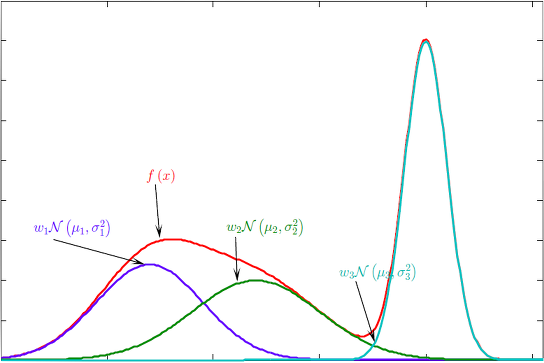
\includegraphics[width=0.65\textwidth]{figs/mixture.png}
	\caption[Caption for LOF]{\emph{The data distribution generated by $f(x)$ can be captured by three normal distribution with various means and variances.}}
	\label{fig:mixture}
\end{figure}

Therefore, the model training process is essentially training and setting up some component ARGs so that all the nodes and edges have the means and variances that best capture the common pattern in the given set of ARGs.\\

Based on the algorithm described by Hong and Huang, we first pick some ARGs from the input sample ARGs, and initialize them as the component ARGs. Then we perform an EM algorithm where on the \textbf{E}xpectation step we run the graph matching algorithm to calculate the matching probability between model ARGs and sample ARGs while on the \textbf{M}aximization step we update the model ARG (e.g. updating means, variances, and deleting redundant nodes) in order to achieve higher matching probability. Finally, once the update is very small, we output the model ARGs to represent the common pattern in sample ARGs:\\

\begin{figure}[h]
	\centering
	\captionsetup{justification=centering}
	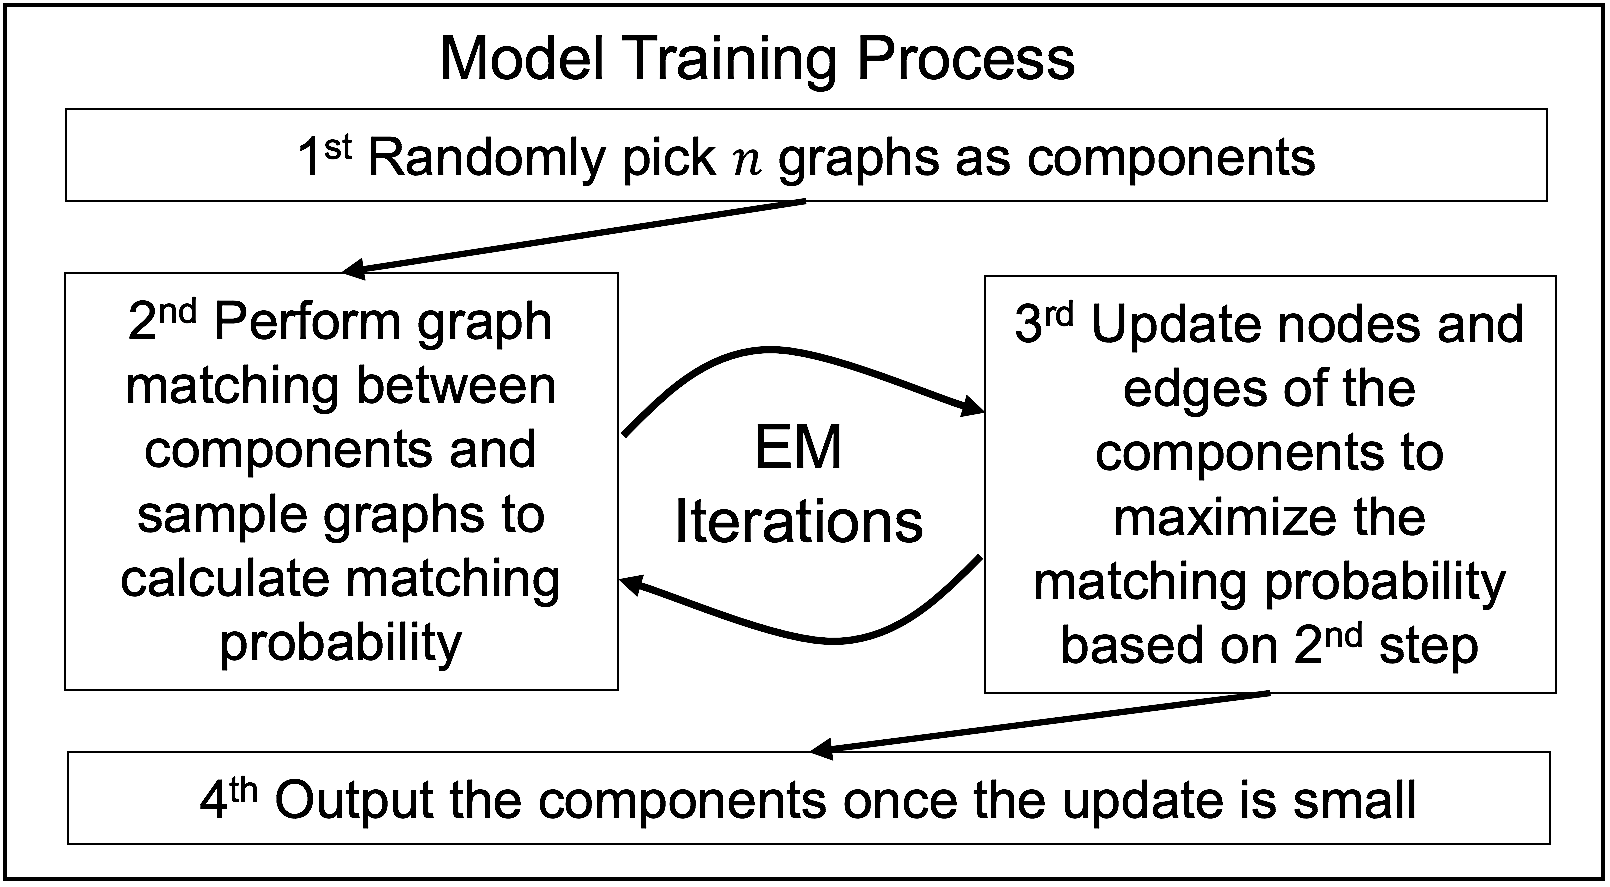
\includegraphics[width=0.8\textwidth]{figs/model_training.png}
	\caption[Caption for LOF]{\emph{The probabilistic parametric model training process with EM algorithm.}}
	\label{fig:model_training}
\end{figure}

\section{Syntax and Definition}

The sample ARGs (i.e. the set of ARGs we want to learn/extract pattern from) is denoted as $\{G_s\}_{s=1}^S$ where $S$ is the number of model components. Within each sample ARG, we indicate the label for each node and edge as $\overrightarrow{N^s_a}$ and $\overrightarrow{E^s_{ab}}$. This is similar to what we have in Chapter \ref{chap: graphmatching} but with an additional index $s$ indicating which sample $G$ these nodes and edges belong to. In addition, we denoted the real nodes in sample ARG, $G_s-\phi$, as $\widehat{G_s}$.\\

For the model, we denoted it as $Z$ and the model consists of a set of parametric model components $\{\Phi_w\}_{w=1}^W$ where $W$ is the number of model components. For each component, there are also an associated weight $\alpha_w$ which indicates how much information the component captures and how important the component is.\\

Within each component ARG, we indicate the mean for each node and edge as $\overrightarrow{N^w_a}$ and $\overrightarrow{E^w_{ab}}$ similar to what we have for sample ARGs, but with $w$ instead of $s$ indicating which model this node and edge belongs to. In addition to the mean, there are also the covariance matrixes for node and edge denoted by $\Sigma^w_a$ and $\Sigma^w_{ab}$ with a similar index. Last but not least, for each node in each component, there is an associated frequency/weight $\beta^w_a$ indicating how important one node is and if we can delete such node.\\

In addition, the matching algorithm introduced in Chapter \ref{chap: graphmatching} can generate match matrix $M^{sw}$ between sample ARG $G_s$ and component ARG $\Phi_w$ as well as the associated node/edge compatibility $C^{sw}$.

\section{Problem Definition}

Given a set of sample ARG $\{G_s\}_{s=1}^S$, our problem will be inferring the parameters in $Z$ including the number of components $W$, weight for each component $\alpha$, mean for each node/edge $\overrightarrow{N^w}$/$\overrightarrow{E^w}$, and the covariance associated with them $\Sigma$.\\

\begin{figure}[h]
	\centering
	\captionsetup{justification=centering}
	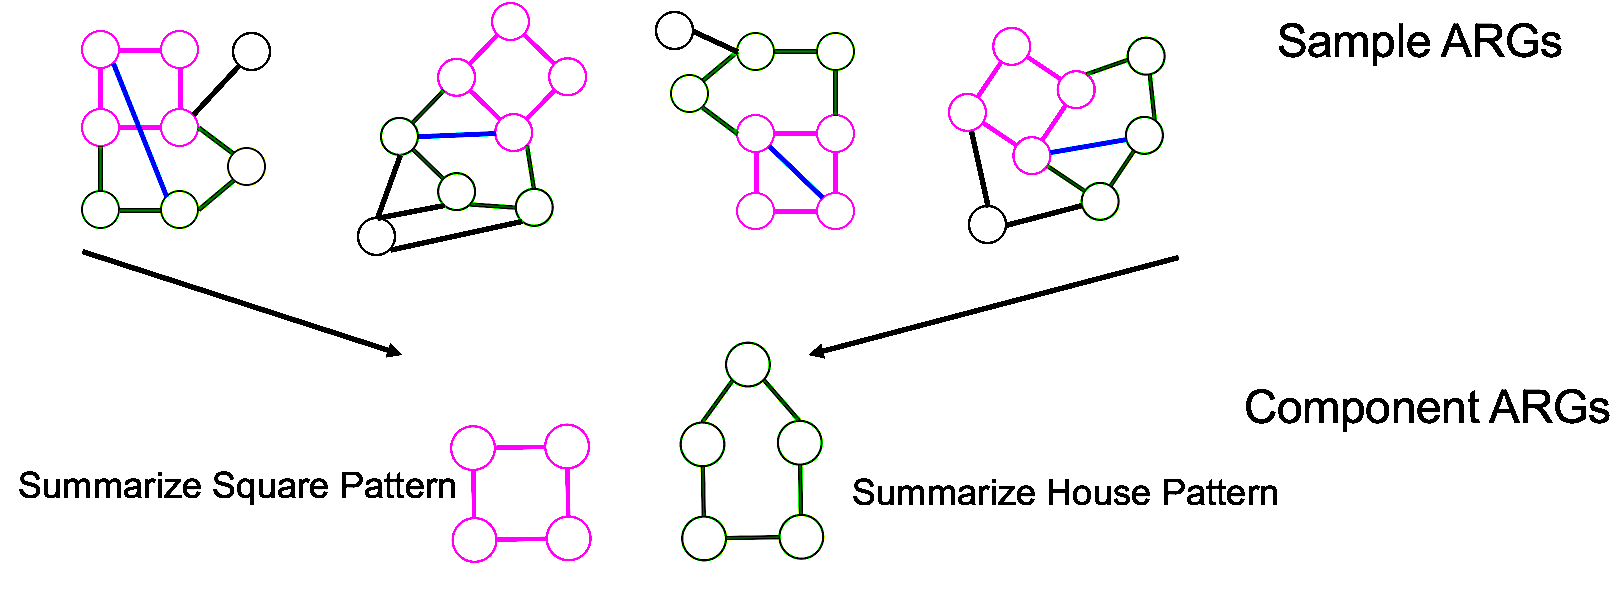
\includegraphics[width=0.8\textwidth]{figs/component_summary.png}
	\caption[Caption for LOF]{\emph{Component can summarize different part of the common pattern.}}
	\label{fig:component_summary}
\end{figure}

\section{Initializing the Components}

The first step of training the model is initializing the components in the model.\\

The way we do is manually pick $W$ random ARG from our sample set, and initialize them as component ARG $\Phi$. We took their original label as the mean, set their covariance matrix as the identity matrix $I$, and give equal weight to all the components and nodes. If we are converting a sample $G_s$ to a component $\Phi_w$, we would have:

\begin{align} 
\overrightarrow{N^w_a} & \leftarrow \overrightarrow{N^s_a} & \forall a \in \widehat{G_s}\\
\overrightarrow{E^w_{ab}} & \leftarrow \overrightarrow{E^s_{ab}}& \forall a,b \in \widehat{G_s}\\
\Sigma^w_a & \leftarrow  I\\
\Sigma^w_b  & \leftarrow  I\\
\alpha_w & \leftarrow \frac{1}{W}\\
\beta^w_a & \leftarrow \frac{1}{|G_s|}& \forall a \in G_s)
\end{align}\\

While we pick $W$ manually based on the complexity of the pattern here, theoretically, we can also start with a relatively larger number of components are delete some of them later. In terms of picking the sample, you can also do better than random by doing a pairwise graph matching among the sample ARG and choose ones that are the most representative based on the match matrixes $M$.

\newpage

\section{EM Algorithm}

Once we initialized the components $\{\Phi_w\}_{w=1}^W$ with all the parameters, we will then run through an EM algorithm to tune this parameters so our model $Z$ can capture the sample $\{G_s\}_{s=1}^S$ at its best. EM algorithm consist of an estimation step where we estimate how well our parameters perform and a maximization step where we tune the parameters to maximize the estimation. We run through these two steps iteratively until the tuning on the parameter is very small.

\subsection{Estimation Step}

In this step we estimate how well model $Z$ representing the sample ARG $G$ as $P(G|Z)$. Once we finish training the model, $f(G_{new}|Z)$ can also be used to predict if a new ARG $G_{new}$ contains the learned/extracted pattern. \\

The first thing we do in the estimation step is matching each component $\Phi_w$ with each sample $G_s$, and get a match matrix $M^{sw}$ from the graph matching algorithm introduced in Chapter \ref{chap: graphmatching}. In addition, the algorithm will also return the node and edge compatibility $C^{sw}$ computed as described in Section \ref{ssec:compatibility}.\\

Once we have the match matrix, we can calculate the probability of $G_s$ matching $\Phi_w$:

\begin{align} 
& \xi(G_s|\Phi_w)=\sum_{a=1}^{\widehat{G_s}}\sum_{i=1}^{\Phi_w}M^{sw}_{ai}C^{sw}_{ai}+ \sum_{a=1}^{\widehat{G_s}}\sum_{b=1}^{\widehat{G_s}}\sum_{i=1}^{\Phi_w}\sum_{j=1}^{\Phi_w}M^{sw}_{ai}M^{sw}_{bj}C^{sw}_{abij}\\
& P(G_s=\Phi_w)=\frac{\xi(G_s|\Phi_w)}{\sum_{t=1}^{W}\xi(G_s|\Phi_t)}
\end{align}\\

With $\xi(G_s|\Phi_w)$, we then can calculate:

\begin{equation} 
f(G|Z) = \sum_{w=1}^W\alpha_w\xi(G|\Phi_w) \label{eq:fgz}
\end{equation}\\

\subsection{Maximization Step}

In the maximization step, we adjust and tune the variable based on $P(G_s=\Phi_w)$, $M^{sw}$ and $C^{sw}$ that we calculated in the Estimation step.

\subsubsection{Update Component Weight}

First we update the component weight $\alpha_w$ for each component $\Phi_w$ as:

\begin{equation} 
\alpha_w=\frac{\sum^S_{s=1}P(G_s=\Phi_w)}{S}
\end{equation}\\

The component weight here is essentially calculating the average probability it matched to all the sample ARGs $\{G_s\}^S_{s=1}$.

\subsubsection{Update Component Node Frequency}

Then we update the frequency (i.e. weight) for each node in each component $\Phi_w$:

\begin{equation} 
\beta^w_a=\frac{\sum^S_{s=1}\sum^{\widehat{G_s}}_{i=1}M^{sw}_{ia}P(G_s=\Phi_w)}{\sum^S_{s=1}|\widehat{G_s}|P(G_s=\Phi_w)}
\end{equation}\\

The component node frequency is essentially an weighted average of the matching probability of this specific component node in all the matching matrix $M^{sw}$.\\

\subsubsection{Update Mean for Component Node}

To tune the mean for each component node, $\overrightarrow{N^w_a}$, we follow:

\begin{equation} 
\overrightarrow{N^w_a}=\frac{\sum^S_{s=1}\sum^{\widehat{G_s}}_{i=1}\overrightarrow{N^s_i}M^{sw}_{ia}P(G_s=\Phi_w)}{\sum^S_{s=1}\sum^{\widehat{G_s}}_{i=1}M^{sw}_{ia}P(G_s=\Phi_w)} \label{eq:nmean}
\end{equation}\\

Here we essentially calculated a weighted average of all the sample nodes, $\overrightarrow{N^s_i}$, based on how likely our component node matches to that sample node in match matrix $M^{sw}$ and how likely the component matches to that sample $P(G_s=\Phi_w)$.\\

\subsubsection{Update Covariance Matrix for Component Node}

Once we update the mean, we will also need to update the covariance matches $\Sigma^w_a$ for the component node:

\begin{equation} 
\Sigma^w_a=\frac{\sum^S_{s=1}\sum^{\widehat{G_s}}_{i=1}\overrightarrow{x^s_i}\overrightarrow{x^s_i}^TM^{sw}_{ia}P(G_s=\Phi_w)}{\sum^S_{s=1}\sum^{\widehat{G_s}}_{i=1}M^{sw}_{ia}P(G_s=\Phi_w)}
\end{equation}
where $\overrightarrow{x^s_i} = \overrightarrow{N^s_i} - \overrightarrow{N^w_a}$.\\

Similarly, here we essentially calculated a weighted average of covariance between the component node and sample nodes, $(\overrightarrow{N^s_i} - \overrightarrow{N^w_a})(\overrightarrow{N^s_i} - \overrightarrow{N^w_a})^T$, based on how likely our component node matches to that sample node in match matrix $M^{sw}$ and how likely the component matches to that sample $P(G_s=\Phi_w)$.\\

\subsubsection{Update Mean for Component Edge}

Similar to how we calculate the mean for component node $overrightarrow{N^w_a}$, we calculate the mean for component edge $\overrightarrow{E^w_{ab}}$ as:

\begin{equation} 
\overrightarrow{E^w_{ab}}=\frac{\sum^S_{s=1}\sum^{\widehat{G_s}}_{i=1}\sum^{\widehat{G_s}}_{j=1}\overrightarrow{E^s_{ij}}M^{sw}_{ia}M^{sw}_{bj}P(G_s=\Phi_w)}{\sum^S_{s=1}\sum^{\widehat{G_s}}_{i=1}\sum^{\widehat{G_s}}_{j=1}M^{sw}_{ia}M^{sw}_{bj}P(G_s=\Phi_w)}
\end{equation}

\subsubsection{Update Covariance Matrix for Component Edge}

Similar to how we calculate the covariance matrix for component node $\Sigma^w_a$, we calculate the covariance matrix for component edge $\Sigma^w_{ab}$ as:

\begin{equation} 
\Sigma^w_{ab}=\frac{\sum^S_{s=1}\sum^{\widehat{G_s}}_{i=1}\sum^{\widehat{G_s}}_{j=1}\overrightarrow{z^s_{ij}}\overrightarrow{z^s_{ij}}^TM^{sw}_{ia}M^{sw}_{bj}P(G_s=\Phi_w)}{\sum^S_{s=1}\sum^{\widehat{G_s}}_{i=1}\sum^{\widehat{G_s}}_{j=1}M^{sw}_{ia}M^{sw}_{bj}P(G_s=\Phi_w)}
\end{equation}
where $\overrightarrow{z^s_{ij}} = \overrightarrow{E^s_{ij}} - \overrightarrow{E^w_{ab}}$.\\

\subsubsection{Delete Redundant Node}

Since we initialized the component from sample ARGs, it is likely that the component itself will have background nodes (i.e. nodes not in the common pattern) that are redundant. To reduce the component ARGs from sample ARGs to the smaller common pattern, we can do node deletion based on the node frequency $\beta^w_a$ and some threshold. For instance, we choose to delete the $a$th node in $\Phi_w$ if:

\begin{equation} 
\beta^w_a < 1 - 0.85^n
\end{equation}
where $n$ indicate the $n$th round of the EM algorithm.\\

However, you can also choose to used a hard threshold like $0.85$ or delete redundant node in the very last round. In addition, we can also choose to delete redundant component here, even though we did not explore such option.

\subsubsection{Converge Condition and EM Algorithm Exit}

At the beginning of the EM algorithm, the maximization step will make large modification on each parameter, so we would go back to the estimation step after finishing the maximization step. \\

However, towards the end of the algorithm, we need to check if the EM algorithm has already converged (changes are small). If so, then we can exit the EM algorithm and go to the next step. Here, we simply compared previous component weight $\alpha^{(0)}$ with the current component weight $\alpha^{(1)}$, and exit if the differences is smaller than some number $\iota$:

\begin{equation} 
\sum^{W}_{w=1}\alpha^{(0)}_w<\iota
\end{equation}\\

However, this is not the only choices, and you can use other converging conditions if you like. Especially when your model only contains one component, you will have to use another condition since $\alpha_w$ will always be $1$.\\

\newpage

\section{Detect the Spatial Pattern}

Once we finished training the model, how do we detect or predict if the extracted/summarized pattern exist in a new ARG? As mentioned above, we can use $f(G|Z)$ calculated by Eq.\ref{eq:fgz} as our similarity score to determine if the new ARG, $G$, contains the same spatial pattern as the training samples. Therefore, we would need to setup some sort of threshold, $\chi$, so that $G$ contains the learned pattern only if $f(G|Z)>\chi$.\\ 

To setup $\chi$, we generate a set of $R$ random graphs $\{G^r\}^{R}_{r=1}$ with similar number of nodes, edge connectivity\footnotemark, and labels as our training sample $\{G^s\}^{S}_{s=1}$. With the random generated ARGs, we can calculate a set of similarity score $\{f(G^r|Z)\}^{R}_{r=1}$ that can help us determine the threshold $\chi$. If you have enough computational power, and are able calculate the similarity score for a very large number\footnotemark of random ARG. You can simply take the $99.99\%$ percentile of the similarity score set $\{f(G^r|Z)\}^{R}_{r=1}$.\\
\footnotetext{How many nodes one node connected to.} 

However, unlike Google\footnotemark, we do not live in a magic land. Therefore, we only calculated the similarity score for $50$ random ARGs and run z-test on the set of similarity scores $S=\{f(G^r|Z)\}^{R}_{r=1}$ which allows us to set the threshold $\chi$ as $\chi \leftarrow \mu+3\sigma$ where $\mu$ and $\sigma$ are the mean and variance of the similarity scores of random ARGs.
\footnotetext{Let's say $R>1,000,000$.}
\footnotetext{https://twitter.com/deliprao/status/842635509255962624}\\

Due to the application of our model, we do not consider the case where a random but much larger graph could potentially score a higher similarity simply because there are more node to sum. Therefore, if your application are dealing with ARGs on a large spectrum of node number, you might need to modify $f(G|Z)$ to factor in $|G|$.

\section{Implementation Detail}

\subsection{Coding Complexity}

While the model introduced here seems to be pretty straight forward, the actual coding is rather tedious since we have many steps, parameters and nested summation. Therefore, we break down the algorithm and modulated each step so it is easier to debug.

\subsection{Null Node in the Model}

While it is not mentioned above, the model we implemented actually has a null node $\phi$, but it does not have any label on the node or edges. Instead, the graph matching algorithm will ignore this null node and used its own null node definition as described in Section \ref{ssec:nullnode}. However, when the graph matching return the match matrix and compatibility, $M^{sw}$ and $C^{sw}$, they include the value for algorithm's own null node which we can used for the model null node. Such implementation allows us to use the graph matching algorithm developed earlier with very little modification and save the troubles of maintaining the parameters for the null node.

\subsection{Run Time}

We trained a model with $2$ components on $5$ pattern embedded ARG with $\sim30$ nodes, and it took $\sim 30$ minutes including the time for setting up the pattern detection threshold $\chi$. As mentioned in Section \ref{ssec:graphmatchingruntime}, you can adjust the parameter for converging condition and learning rate to tradeoff between accuracy and running time.

\section{Testing the Model}

Similar to how we generated test cases in Section \ref{sec:graphmatchingtest} for graph matching algorithm, we generate a set of ARGs with ($G^p$) or without ($G^r$ i.e. random ARG) the embedding pattern. \\

Then we train a model on some of the ARGs with the pattern (i.e. $G^p$) and plot a histogram of the similarity score ($f(G|Z)$) for all $G^p$ and $G^r$. This is a sample result generated by a set of ARGs with $\sim30$ nodes, and the model is trained by $5$ sample ARGs with $2$ component ARGs.:

\begin{figure}[h]
	\centering
	\captionsetup{justification=centering}
	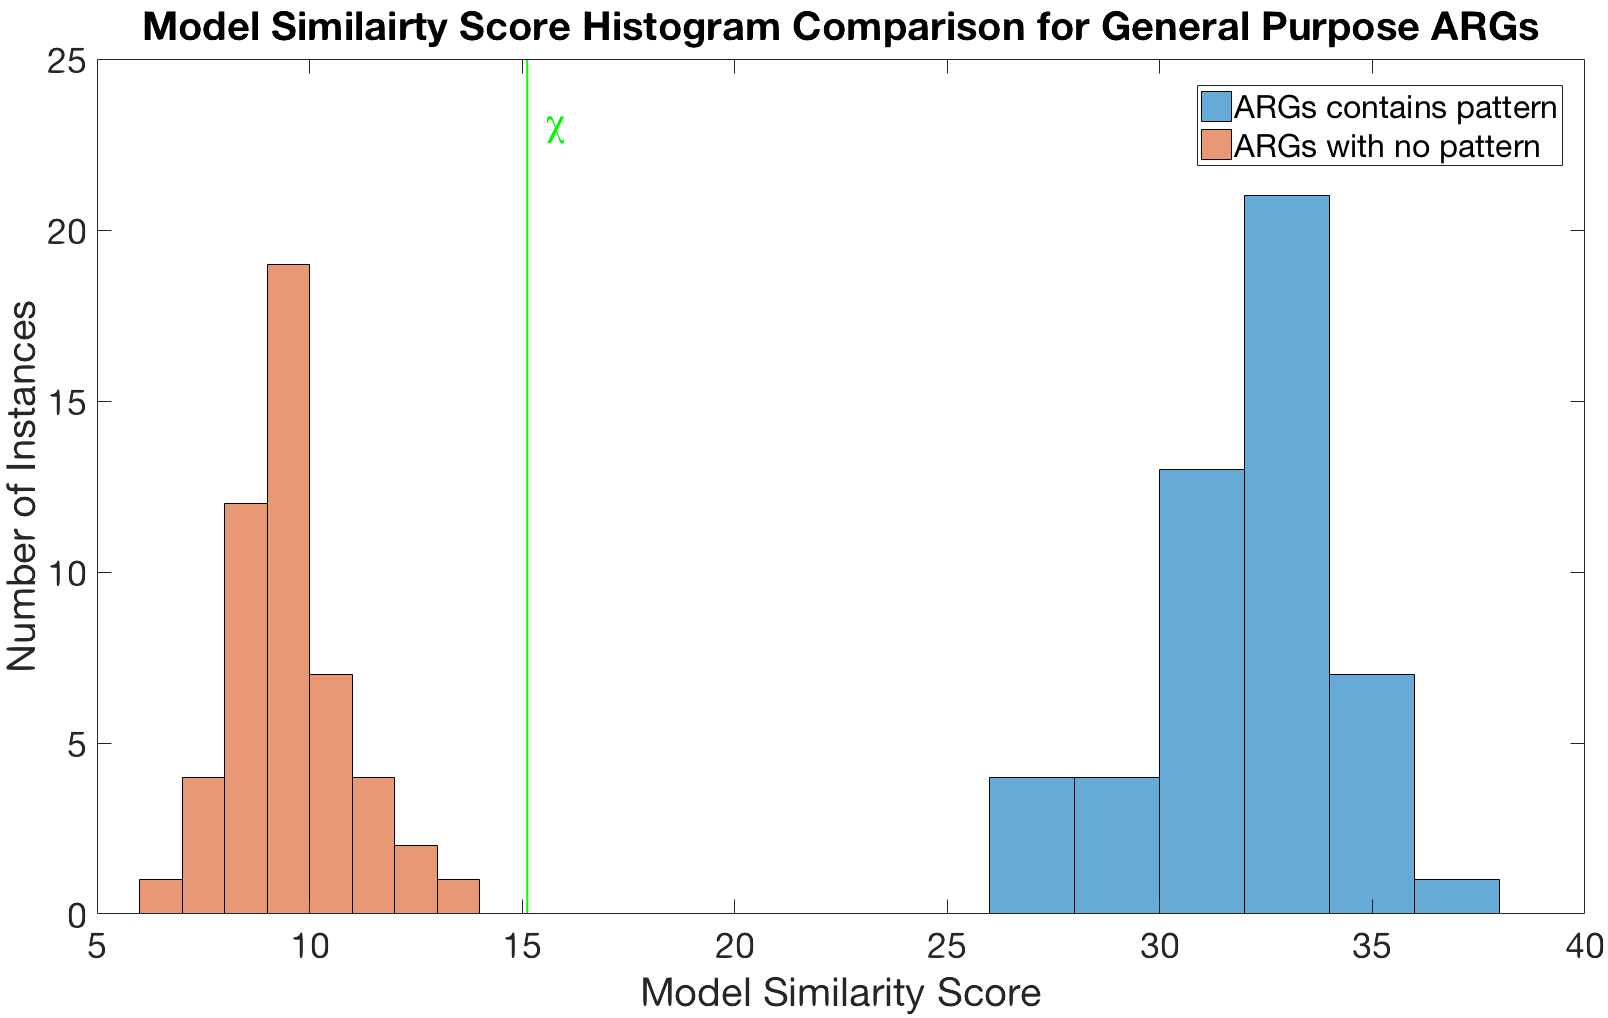
\includegraphics[width=0.9\textwidth]{figs/pattern_learning.png}
	\caption[Caption for LOF]{\emph{Similarity Score $f(G|Z)$ for pattern embedded ARG (blue) and random ARG(orange) while the green vertical line is the threshold $\chi$.}}
	\label{fig:pattern_learning}
\end{figure}

\section{Conclusion}

In this chapter we introduced a probabilistic parametric model $Z$ that we can train via EM algorithm. This model allows us to learn the common/share pattern among a set of ARGs, and used a set of component ARGs to represent/summarize such pattern. By calculating $f(G|Z)$ and comparing it to the threshold $\chi$, we can predict if a new ARG $G$ contains the learned pattern.\\

If we can model a protein crystal structure as an ARG, we can potentially use this model to mine novel protein structure or functional structure from protein crystallography data.









% \chapter{Cycles as a Vertex Invariant}

A powerful feature of the Cycles invariant is that it cannot only discriminate between graphs, it has structure which naturally suggests mappings between their vertices which have the potential to be isomorphisms.
This section will discuss exactly how isomorphisms can be constructed and evaluated by using cycles as a vertex invariant.
Central to this chapter is the concept described earlier as Automorphism Equivalence Classes, or Similar Vertex Sets (SVS).

\section{Similar Vertex Sets}
\label{section:qsvsesdef1}

A vertex-similar set is a subset of the vertices of a graph such that for any pair of vertices in the set, there exists an automorphism which maps one to the other.
Note that vertex similarity is reflexive (as one-to-one mapping (such as an automorphism) is invertible). 
Also note that membership in vertex-similar sets is transitive (as we can simply use the `followed-by' operator on the component automorphism mappings).

Thus, all vertices in a graph can be partitioned into some number of similarity-sets, where every set has at least one element, and the union of the sets is the vertex set.
It is the structure of these disjoint, covering sets, each of which is internally vertex-similar which we will call Similar Vertex Sets, or SVSes for short.
When we are referring to a single vertex-similar set, we will say `an SVS', and when we are referring to the covering structure of multiple, disjoint, covering sets, we will refer to them as the `SVSes'.
For the sake of simplicity, we will assume that there is some well-ordering over these sets, so that we are able to assign an order between each SVS within the SVSes.
In practice, this will be a practical function of how we go about computing the SVSes.

This construction is deeply tied to isomorphism checking and discovery.
If we have two graphs $G$ and $H$, and their Similar Vertex Sets are $SVS(G)$ and $SVS(H)$, based on the size of each set, we have a maximum number of potential isomorphisms.
First off, if we examine every $i$th paired set between $SVS(G)[i]$ and  $SVS(H)[i]$, if the sizes of the sets differ, then we can immediately reject the possibility of isomorphism between $G$ and $H$.
If the size of each component set are the same, we can check for isomorphism by brute force, by calculating every possible permutation between the paired sets, and then every combination of those permutations across all of the SVSes.

One should note that this is simply a way of describing the end goal of a vertex coloring (where like-colored vertices are automorphic to one another).
SVSes are easier to discuss concretely within the context of Cycles, and have the additional feature that we allow them to be imperfect, or defined by a particular facet of the graph/invariant.

Though we can make many practical arguments which greatly simplify the number of these possibilities we have to test for isomorphism, it should be noted that in the overwhelming majority of cases, this simple algorithm only has to check \emph{one} mapping for an isomorphism.
This is by virtue of the fact the the overwhelming majority of graphs have only a single automorphism.

\section{Most Graphs Have One Automorphism}

This is by virtue of a simple fact: we can talk broadly about the average number of automorphisms in a set of graphs, and even better, we can calculate precise means for the average number of automorphisms for graphs of a certain size.
Remember that the number of undirected, non-looped, single-edge graphs (or as we have just been calling them, graphs), over $N$ vertices has a known closed form.
We also know that the number of graph instances over $N$ nodes is simply the number of undirected matrices over $N$ nodes, $2^{E_{max}}$.
Finally, we know that the number of matrices 

$$ M_{reps}(g) = \frac{N!}{|Aut(g)|} $$
$$ \sum_{g \in G_{alg}} M_{reps}(g) = \sum_{g \in G_{alg}} \frac{N!}{|Aut(g)|} $$
$$ 2^{\frac{N^2 - N}{2}} = N! \sum_{g \in G_{alg}} \frac{1}{|Aut(g)|} $$
$$\frac{\sum_{g \in G_{alg}} \frac{1}{|Aut(g)|}}{|G_{alg}|} =  \frac{2^{\frac{N^2 - N}{2}}}{N! * |G_{alg}|} $$
$$ \xoverline{|Aut^{-1}(g)|} = \frac{2^{\frac{N^2 - N}{2}}}{N! * |G_{alg}|}$$

Though we don't have a closed form for this, a quick calculation pretty easy, and gives us a very clear trend.
In figure \ref{fig:mostgraphsoneaut}, there are two figures shown.
The first plot shows the right hand side of the final equation, graphed for different values of $N$.
The second plot explores the difference between the first plot and one, and takes the logarithm to see how small the values get.

\begin{figure}[h]
\caption{\emph{Most Graphs Have Exactly One Automorphism} - It is clear that as $N$ increases, the right hand side of our above equation approaches 1. Not only that, but it appears to do so exponentially fast.  The plot on the right shows a logarithmic linear approach to one.}
\centering
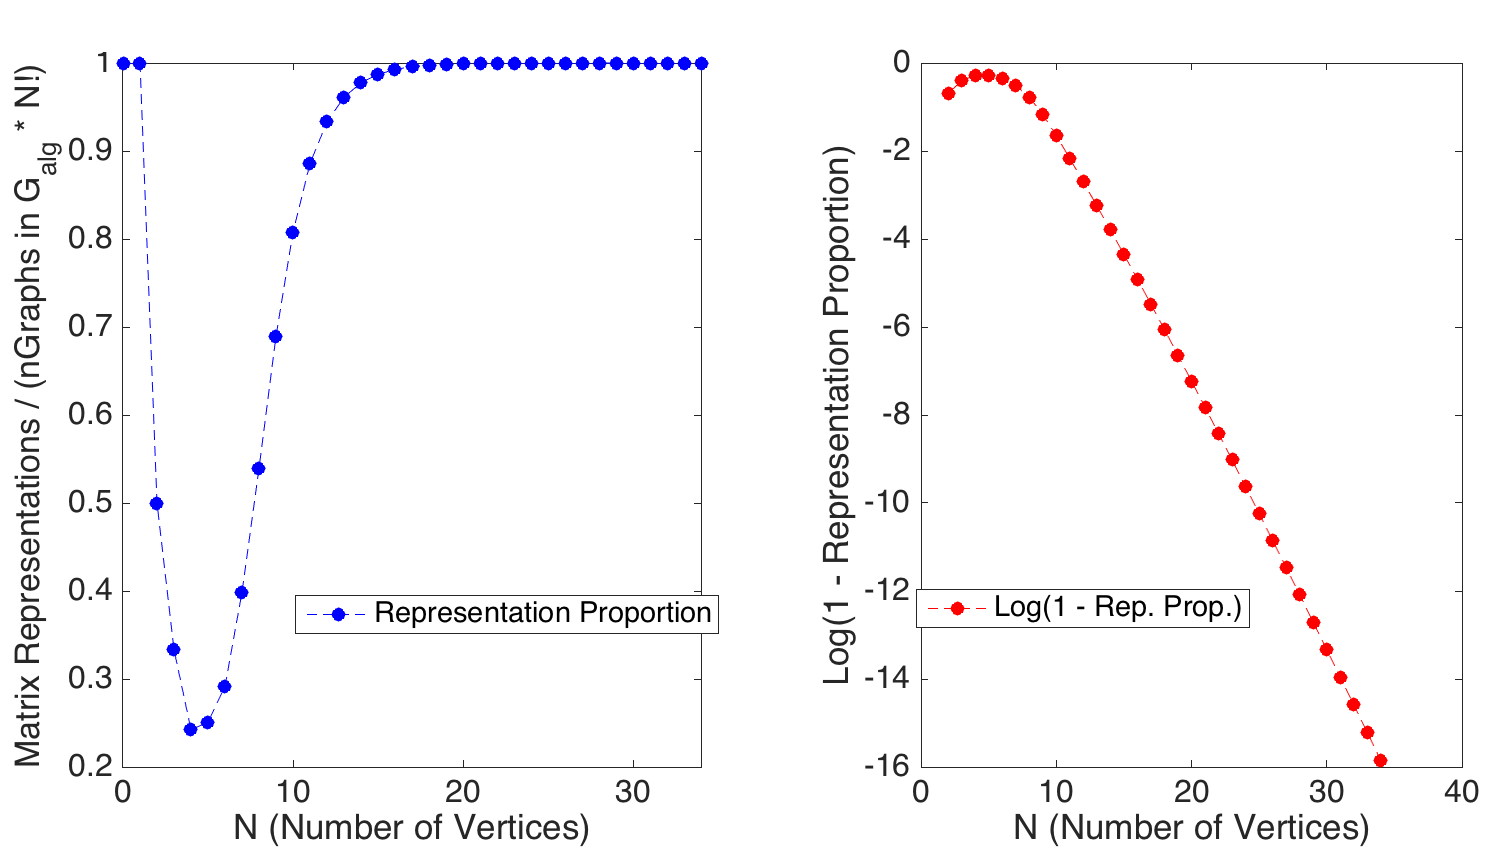
\includegraphics[width=\textwidth]{numGraphsAndMats}
\label{fig:mostgraphsoneaut}
\end{figure}

This should convince even a skeptical reader that for an average graph $g$ (even when treating it like an algebraic object), as $N$ increases, $\xoverline{|Aut(g)|} \rightarrow 1$.

\subsection{Implications for Perfectly Similar Vertex Sets}

Applying this back to our original purpose, we can surmise that the proportion of graphs which have only the trivial automorphism increases to one as $N$ increases.
In this common case, the SVSes are a set of $N$ distinct, one element sets, where each vertex is distinguishable from each other, and none share any automorphisms.
This makes checking for isomorphism between two random graphs trivial (if we have the SVSes), as the overwhelming majority of the time, we will only need to try the isomorphism implied by the direct, one to one mapping between the SVSes of the two graphs.

However, checking for automorphisms between every single pair of vertices is clearly in a higher computational complexity class than testing for isomorphism.
Thus, we will use smart heuristics to develop quazi-similar vertex sets, which will enable us to get the benefits of SVSes (i.e. implying the isomorphisms to try) without actually proving that the automorphisms that define the SVSes exist.

\section{Quazi-Similar Vertex Sets}

Quazi-Similar Vertex Sets (QSVSes) are constructed with respect to a vertex invariant, but have the same structure as SVSes.
The vertex invariant is calculated for all vertices within the graph, and those with the same value are placed into the same set.
Transitivity and reflexivity clearly both hold under this definition.
Moreover, the ordering/comparability of vertex invariants gives us a natural way to order the sets within the QSVSes.

In this section, we will describe how using the cycles invariant to generate QSVSes is highly successful at mirroring the true SVSes, and suggest an augmentation to cycles which correctly differentiates the two for a high proportion of cases.

\section{Why $P^*(G) <N$: Limitations on Cycles Usefulness}
\label{section:pstar}

\subsection{What is $P^*$, why does it matter?}

An ENORMOUS part of this thesis has thus far gone as assumed: what is $P$ (the maximum length cycle we are considering)?
When we are discussing cycles through a node, how long are the cycles we are considering?
The vertex invariant for cycles is clearly a vector, with the length of cycles corresponding to the place within the vector (cycles of length 2, 3, 4, etc.), but where do we draw the line?
To answer this question, I used a notion of `usefulness', to maximize the amount of information that we get out of the cycles invariant for the computation that we put into it.

Specifically, within the context of cycles as a vertex invariant, I started out with the assumption that all vertices share a single Similar Vertex Set (i.e. all are similar unless we have proof that they are not).
We then distinguish vertices by advancing P by one, we are in effect splitting this one class (or smaller classes) into even smaller classes, based on the information gleaned by increasing the length of all invariant vectors by one.
This kinds of `breaking-down' leads us to a concrete notion of usefulness: for a given graph G, cycles is useful at a power $P^*(G)$, where $P^*(G)$ is the minimum value for P at which all of the vertex sets in the SVSes are as broken down as they can get (for any larger values of P).
Thus, if we take the maximum of $P^*(G)$ across the set of all graphs over $N$ vertices and $M$ edges, , we will find a value $P^*(S_{N,M})$ at which point computation beyond this point is redundant for graphs over this set of graphs.
In this section we will be ignoring $M$, and examining the critical value for P over all values of $M$ while fixing $N$.
This would enable us to more concretely talk about running time, and its tradeoffs as a function of $N$ alone.
What we find (through both computational exploration and theoretical justification) is that $P^*(S_{N})$ can be described in direct terms of $N$:

\[ P^*(S_{N}) = \begin{cases} 
      N-1 & \text{If N is odd} \\
      N-2 & \text{If N is even} \\
   \end{cases}
\]

\subsection{Observational Data: Diameter vs. $P^*(G), G \in S_N$}

I first examined $P^*(G)$ as a function of the individual graph $G$, rather than over the set of all graphs, to try to see how the overall distribution of $P^*(G)$ looked for all graphs in the set.
Though this did not lead me anywhere directly, it did give me a clear idea of the upper bounds on $P^*(G)$ for an individual graph.
Shown in figure \ref{fig:diamvsmaxpower} is a description of this relationship.  By no means is it rigid, but the correlation is very strong between diameter and $P^*(G)$, labeled as $P_G$ on the y-axis.
It is also interesting (personally) just to see the diameter of a set of graphs laid out like this.

\begin{figure}[h]
\caption{\emph{Diameter Against $P^*(G)$ with $N=9$} - The size and number next to each circle tell us how many graphs (as algebraic objects) fit into different sizes of diameter and $P^*(G)$, labeled $P_G$}
\centering
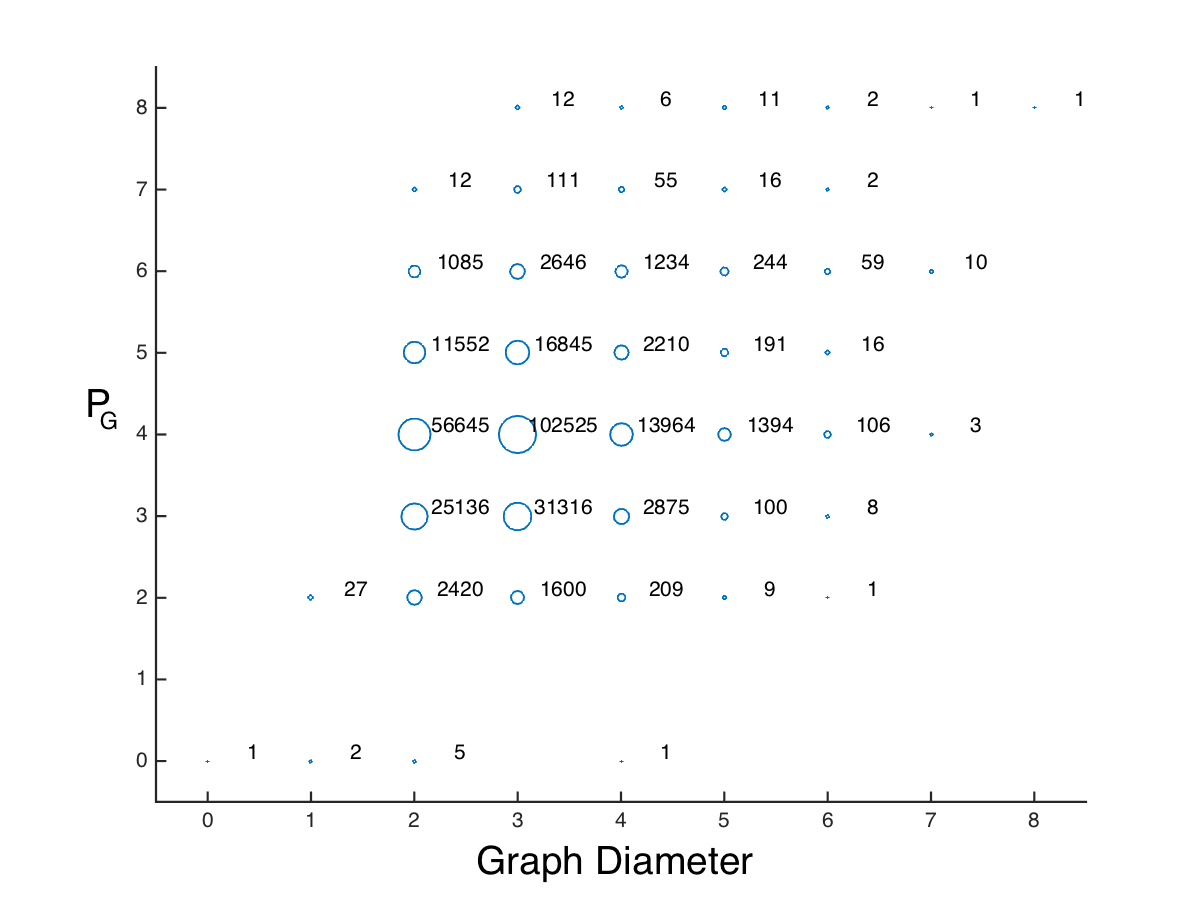
\includegraphics[width=\textwidth]{N9DiamVsDiffPower}
\label{fig:diamvsmaxpower}
\end{figure}

Four things are consistent across all of the alike graphs (shown in an appendix):
\begin{itemize}
\item{There is consistently a maximum diameter for $P^*(G)$, implying a $P^*(S_N)$ for each as shown in the table below}
\item{There are never any graphs with $P^*(G) = 1$, as we do not allow self loops }
\item{The Path graph ($P_N$), is always the lone member of the far upper right hand corner}
\item{The Cycle graph ($C_N$), always has $P^*(G)$ equal to that of the Path graph: $P^*(C_N) = P^*(P_N)$}
\end{itemize}
The upper bound proposed by each one of the values for $P^*(S_N)$ follows the pattern:
\[ P^*(S_N) = \begin{cases} 
      N-1 & \text{If N is odd} \\
      N-2 & \text{If N is even} \\
   \end{cases}
\]
for $N <=9$. This sets up a strong case for this as a target hypothesis, but we still must prove it.

\subsection{Theoretical Justification: $P_N$ versus $C_N$}
Why does the proposed value for $P^*(S_N)$ make sense?

This proof consists of two parts, the first is why $P^*(P_N) = \text{the proposed} P^*(S_N)$ for the Path graph ($P_N$), the second describes why all other graphs $G$ have $P^*(G) \leq P^*(P_N)$.

Part 1: \emph{Distinguishing between vertices in the path graph requires $P^*(P_N) = N - 1 - ((N+1)\%2)$.}

Start all vertices in the same assumed similarity set, and assume that $P = 0$.
When we increase $P$ to 2, all vertices have degree 2 (the second entry in the cycles invariant) except for the two terminuses, thus the two terminuses are split off from the original quazi-similarity set, as they have been distinguished at $P=2$ by their cycles invariant.
When we increase $P$ to 4, the two nodes adjacent to the two terminuses are now distinguished (as they are now `missing' a path of length four that they would have had if they were further in toward the center of the path graph). 
There are now $N-4$ vertices remaining in the original quazi-similar vertex set.
From this, it is clear to see that for an arbitrarily large path graph, for $P=2K$, there will be $N-2K$ elements in the original QSVS.
We will have \emph{fully distinguished} all of the vertices into distinct QSVSes which are true to the SVSes when the original QSVS contains only the `middle' node(s).

In the even case $N = 2K, K \in Z$, this occurs when we have 
$$P^*(P_N) = 2\ceil{\frac{N-2}{2}} = 2\ceil{\frac{2K}{2} - 1} = 2\ceil{K - 1} = 2(K - 1) = 2K - 2 = N - 2$$
In the odd case $N = 2K +1, K \in Z$, this occurs when we have 
$$P^*(P_N) = 2\ceil{\frac{N-2}{2}}  = 2\ceil{\frac{2K+1- 2}{2}} = 2\ceil{K - 1/2} = 2K = N - 1 $$

Thus, we know that 
\[ P^*(P_N) = \begin{cases} 
      N-1 & \text{If N is odd} \\
      N-2 & \text{If N is even} \\
   \end{cases}
\]

Part 2: \emph{Why is $\forall g \,\in\, S_{N} , \;P^*(P_N) \geq P^*(g)$? Why is the path the hardest to internally distinguish?}

Cycles invariant calculation is a form of vertex coloring for isomorphism testing, with the feature that distinguishes vertices being the number of cycles that pass through them of given lengths.
Since $P^*$ is concerned with the largest value of Cycles able to all nodes from one another internally, we know that the graph that is the hardest to internally distinguish will (1) at least have two distinct groups (if not more) of vertices within it, and (2) will have a slow traversal of its colorings (which is a function of its girth, the maximum distance between two nodes in the graph).
If we can distinguish any pair of vertices from one another at any level (if at the degree sequence, at P=2, or at the number of triangles, P=3, etc.), then we can distinguish the vertices which are only attached to one of the pair members that we distinguished at $P+2$, as that new cycle will be reverberated to the connected vertices with cycles that can traverse to the distinguished node, complete the cycle, and return back.
Thus, cycles, propagates in such a way that whenever we can make a single distinction of two nodes (say $v_j$ and $v_k$) in the graph (lets say at $P=p_0$), then all nodes in the graph will be as distinguished as they are able to be via Cycles at $P=K+2*max\big[min\big(dist(v_i,v_j), dist(v_i,v_k)\big)\big]$.
It is clear that the maximum value of the maximum term is half the value of the girth of the graph (as in the worst case, $v_j$ and $v_k$ are the vertices that are furthest apart, defining the girth, and the distance between $v_i$ and one of the two vertices is maximized when $v_i$ is equidistant from each. 
Thus, we can change this expression into $P=K+girth(G)$.
Meaning there are two different ways to try to maximize this expression with respect to P (as that is what we are really trying to find), we could either try to maximize it by maximizing the girth or by maximizing K.
Since K is a function of the first feature that can be distinguished, it is clear that $K$ will be strictly less than $N$ (as if we get to that point, then we will not be able to make any distinctions).
Thus, the way to maximize $P$ is to maximize the girth.
This occurs in the path graph ($P_N$).
Thus no graph can have larger $P^*(G)$ than the path graph.

The combination of these two claims proves that the expression 
\[ P^*(G) \leq \begin{cases} 
      N-1 & \text{If N is odd} \\
      N-2 & \text{If N is even} \\
   \end{cases}
\]
holds for all graphs, a useful piece of knowledge in curtailing the amount of computational work we must do, and is a novel result within the literature around the $Cycles$ Invariant. 

\section{Improving upon QSVS with Flagged Cycles}

This section deals heavily with definitions of QSVSes defined in sections \ref{section:qsvsesdef1} and \label{section:qsvsesdef2}.
The quality of the QSVS is generally described as how close they are to the true SVSes.
In other words, quality is a measure of how frequently does a QSVS contain two or more subsets that should be independent SVSes.
Though Cycles as a vertex invariant produces QSVSes which mirror SVSes with high probability, we should examine the failures cases to see if we can do better.

We will accomplish this via a methodology I am calling `flagging' after I have seen that a few times in the literature.
Flagging (or Marking) is the process of taking a graph and appending a single vertex to it which is connected by a single edge to some target vertex in the graph.
Flagging frequently modifies graph structure enough to see impacts which successfully differentiate between non-isomorphic/non-automorphic structures.

For example, if we have two co-spectral graphs, and we are curious whether or not an isomorphism exists between the two of them, we can append a flag on each one of the vertices which must be mapped together in a potential isomorphism, and then take the chromatic polynomial again.
If the new (flagged) graphs differ in their chromatic polynomial, then the two vertices that were flagged cannot have an isomorphism to one another, as modifying two isomorphic graphs in a systematically consistent way should preserve isomorphism.
We use this principle in the pursuit of fully differentiating a set of QSVS into a refined state that is more likely to equal the ground-truth SVSes.

\subsection{Appending a Flag, Somewhat Predictable}

Our methodology for modifying the QSVSes is simple: first, calculate the QSVSes using the Cycles invariant.
For each of the sets within the QSVSes with more than one element, perform a flagging operation K times, if the set has K elements, which results in K different graphs.
Calculate the cycles graph invariant over each of these graphs.
If the cycles invariants for any two of the K graphs differs, then split apart the set of vertices into two (or more) new QSVSes, one for each different value of the graph invariant associated with the graph formed by flagging each vertex.

An interesting piece of this is that we can actually predict some of the values that the newly created, flagged graphs, will have for their cycles invariant values.
Specifically, if we are given the previous value of the cycles invariant, and told which vertex in the cycles invariant is going to be appended to, we can predict the number of cycles for the flag vertex (the new vertex), as each one of the cycles that it is a part of must go to and from the flagged vertex (the vertex the new vertex was attached to), and we already knew how many of those there were from the original cycles function.
Additionally, we can predict the change in the number of cycles for the flagged vertex, as we knew its cycle profile before, and the addition of a single vertex on to it can be interpreted as a recursive definition, where cycles are broken into components that travel back (and forth) from the flag vertex and those that exist within the graph.
Though difficult to explain via formulae and words, I would encourage a skeptical reader to check out my code at (/Thesis/Matlab/constituentpaths/predictPathsOfAddingOneVertex.m).

Equally interesting (to the fact that we \emph{can} predict Cycles for these two nodes when just given the Cycles invariant) is that we \emph{cannot} make any further predictions about the flagged cycles values based solely on the plain cycles values.
We know this to be true because in Co-Cycles graphs, we frequently get different flagged cycles graph invariants when we flag vertices which are suggested to be isomorphic (but are not).
This is a good piece of information to know because it gives us proof that flagging is not some kind of manipulation of information that we already have, it represents a way to get pieces of information that include additional structural information.

\subsection{Intuitive Justification for Flagging}

This section is not grounded in proof, but gives a conceptual reason that flagging works at further discriminating between vertices that we think might be automorphic.
Cycles is really a rough description of the `neighborhood' of a vertex within its context in the graph.
Cycles tells us about the way that the structure reverberates, it is, in many ways, a description of resonance.
One conceptual tool I like is to think about electricity flowing (bidirectionally) around a circuit, and measuring the self-connectivity or resistance between points based on the number of ways that electrons could flow.

Flagging a node changes that resonance.
It changes it in a way that we understand and can predict for the flagged vertex and the flag vertex.
However, it also changes the way that cycles `reverberate' through the flagged vertex, and in doing so, changes the cycles invariant at other vertices.
We can even think of this in more concrete terms: take the cycles invariant for the flagged graph (without sorting), then subtract off the cycles invariant for the non-flagged graph (again, without sorting).

This tells you exactly how many new cycles have been created which pass through the flagged node at least once.
We call this modified matrix the \emph{excess cycles} matrix.
Note that this is \emph{not} the same as the row for the flagged cycles matrix, and actually encodes significantly more information (the constituents of those cycles, not only that they exist).
In doing so, we actually get tangible information about the connectivity of each of the nodes.
From the excess cycles matrix, we can calculate the distance between the flagged vertex and each of the other vertices in the graph.
We can calculate the relative makeup of each of the added cycles (how many pass through each vertex, and how many times does each double back on itself), among a large number of other features.

The intuitive justification for flagging is compelling, and if I had another month to puzzle away at this problem, this is probably the area I would spend the most time focusing on.

\subsection{Analytical Support: Strength of Cycles as Vertex Invariant}

The analytical support for flagging is strong:
for all graphs of size $N < 10$, cycles with flagging as a mechanism for QSVS generation correctly generated QSVSes which perfectly estimated (without flaws) the accurate SVSes.
Few examples were found for $N \geq 10$, though some were.

To give the reader an idea of how useful Cycles (and flagged Cycles) are at discriminating between vertices in graphs, I performed some random trials to attempt to estimate their failure rate.
By failure here, I mean the probability that the QSVSes generated by the invariant are \emph{not} equal to the SVSes that can be found via brute force/automorphism examinations.
Note that this kind of failure is only a lack of perfect distinction, it never means a false negatives, in similar vertex testing false negatives are impossible by either methodology.

In figure \ref{fig:proportionQSVSeqSVS}, you can see the results of a trial which generated 1,000,000 random graphs of size 10, 11 and 12, and calculated the proportion of each that are fully distinguished into their correct Similar Vertex Sets by each methodology of generating them.
What we find is that it appears that as the number of vertices increases, the overall number of graphs which fails this metric decreases, a valuable result.
Additionally, we see that the overall number which fail is very low, which is heartening, and gives us good reason to believe that these are both high quality vertex invariants.

\begin{figure}[h]
\caption{\emph{Proportion of all graphs where SVSes = QSVSes generated by two Methodologies}}
\centering
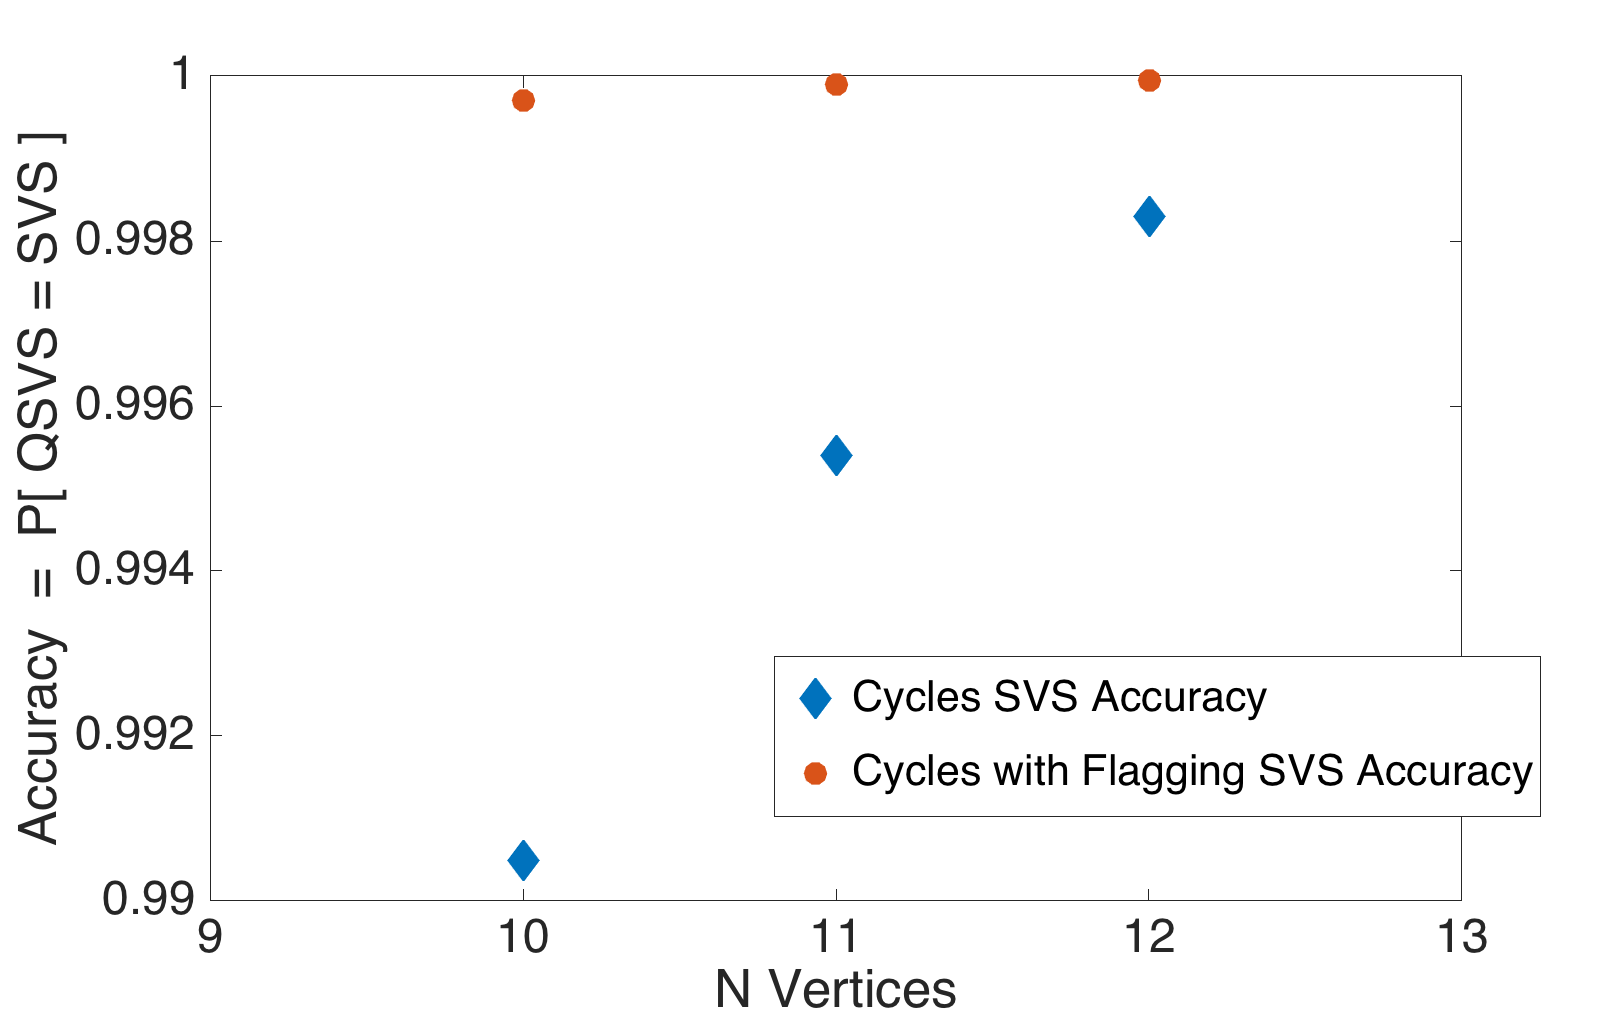
\includegraphics[width=\textwidth]{proportionExploredv10to12}
\label{fig:proportionQSVSeqSVS}
\end{figure}





% \chapter{Canonical Labeling Using Cycles}

A canonical labeling of a graph is a labeling of edges in a way that is consistent across all isomorphic graph instances of the same graph.
Given two graphs and their canonical labelings, graph isomorphism is then a simple quadratic-time check to make sure that alike-labeled vertices preserve all adjacencies and non-adjacencies. 
Thus, any canonical labeling algorithm cannot be in a complexity class smaller than $GI$, the time complexity class of the graph isomorphism problem.

Many parts of my coding projects required the use of a canonical labeler.
Sometimes this was because I wanted to check for isomorphisms on a broad set of graphs, a problem that is possible to complete quickly given the lexicographical nature of canonical labels.
Though there exist good algorithms for determining canonical labeling, I wanted to create my own, both as an exercise in implementation, and in algorithm design.
The result of this process is an algorithm which is relatively slow, but whose time growth is small relative to faster algorithms, due to the relatively large amount of computational work that is done regardless of the difficulty of the graph.

\section{Start With A Vertex Invariant}

The fundamental unit of computation that drives a canonical labeler with this algorithm is a vertex invariant.
For the canonical labeler that I created, I used the flagged cycles vertex invariant, which is described in the third chapter.
Understanding the canonical labeler is not contingent upon an understanding of this vertex invariant, however it is a strategic choice that is rooted in finding a good use for the cycles invariant.

What this does for us is simple, it allows us to directly measure and compare the use of cycles as a vertex invariant to others within a time/power tradeoff.
The result is a canonical labeling algorithm that has much higher constants than its established counterparts, but has a comparably lower time growth rate. 
This is a direct reflection of the quality of Cycles with flagging as a vertex invariant.

\section{A Consistent Algorithm}
The algorithm has a simple interpretation. 
It divides all of the vertices of the graphs into disjoint (covering) sets (QSVSes) based on the value of the cycles vertex invariant.
For each of these sets with more than one vertex, a second round of `flagged cycles' is performed to further divide sets, if possible.
It sorts each of these classes by its size, then by its cycles values.
Each of these sorts is performed in a consistent way, which is irrespective of the original labeling of the graph.

These sorts optimize the interrelationships between vertex sets, so that we are likely to eliminate lexicographically small matrices before even testing them.
This is a version of exponential decision tree pruning, and how the order of the decisions can make pruning easier or harder.
While maintaining our lexicographical target, we are able to significantly reduce the number of checks that are necessary (on the order of $N!$, in the best case).

Once the order of the sets is sorted, we consider every possible permutation of the values within each of the sets so that every possible ordering of vertexes is possible, with the constraint that each set element remains in the higher level order established by the sets themselves.
We start by examining a specific QSVS, and its associated permutations.
We traverse through these permutations and select the matrix which is lexicographically the `smallest', within the context of the already established graph, if some has already been established.
We then add this piece to the growing graph (selecting all `lexicographically maximal' representations), and move on to the next set within the QSVS.
This step-wise pruning means we minimize the overall number of permutations that we test, though it is possible that we accept multiple permutations after a given step of this process is done.
In the final step, we may have multiple permutations remaining (over all the vertices now), but in this context, every permutation will produce the same matrix representation.

I wrote and optimized the algorithm for Matlab (as that is the slowest of my use cases, so having fast code makes a big difference), but then worked on implementing it in C and Javascript (though I didn't go to the same lengths to do the tree pruning).
All three versions of this code are available in my online repository documenting my thesis work.
The Matlab code provides detailed explanations of each piece of the code, why I implemented it that way, and the thoughts that went into it.

The result is quite pleasing, and (alongside a memoization mechanism that saves all results that take longer than 1ms to calculate), canonization of graphs does not bottleneck my computations (even when I am doing millions a minute), despite it being the only computation that I use that operates in exponential time.

\section{Computational Complexity}

There are several factors which contribute to the average case running time of this algorithm, but its worst case is simple to compute: a perfectly automorphic graph, where $|Aut(G)| = N!$.
In such a case, we will perform the original Cycles computation ($O(N^2)$), the secondary flagged cycles calculations ($O(N^3)$) and then a factorial number of checks on the number of remaining isomorphisms ($O(N!)$).
Thus the worst case running time is clearly in factorial time ($O(N!)$).

However, in the average case this is a much less grim scenario.
If we assume (as we have reason to believe) that our flagging algorithm correctly determines SVSes, then our algorithm becomes a function of the number of automorphisms of our graph, in addition to the running time of the flagged Cycles algorithm $(\Theta((|Aut(G)| +1) * N^2))$.
As we have seen in chapter six, the average number of automorphisms in G approaches 1 as $N$ increases. Thus, for sufficiently large $N$, the average running time is on the order of $\Theta(N^2)$.

\section{Time Growth Comparisons to Faster Algorithms}
Any discussion of a homegrown algorithm would be either incomplete or intentionally salacious without a discussion of how it compares to out of the box algorithms.
For these benchmarks, I established two datasets, one of 10000 randomly generated graphs of size ten to fifty using an Erdos-Renyi/Gilbert model, and one using a graph model which is more likely to produce highly automorphic graphs (discussed in detail in chapter 6).
For both of these models we used a probability of $p=0.5$, as these are typically the graphs that are hardest to discriminate against.

To give perspective to my own time results, I used an established and well optimized piece of code, the canonical labeler from the NAUTY package.
A summary of the results is shown below, alongside equations which estimate their overall running time with the above parameters.
From these figures it is clear that the NAUTY package outperforms my canonical labeler, but that my labeler appears to have a lower growth rate.
I would imagine that this difference can be attributed to the large lengths my labeler goes to to minimize the number of permutations that are checked.
NAUTY's algorithm uses simpler heuristics to eliminate permutations, while mine uses significantly more power to make likely better informed choices, at much large computational expense.


% \chapter{Random Graph Generators and Automorphisms}

\section{Random Graph Models}

The field of random graph theory was started with two independent papers in 1959, each defining models for generating and analyzing random graphs.
A \emph{random graph model} is any system of generating graphs with the influence of chance, with various constraints that describe the desired properties of the resulting graphs.
These two papers began a trend in graph theory that allowed theoreticians and algorithm designers to think about efficiency differently, particularly on NP-Hard and NP-Complete graph algorithms.
Rather than concerning themselves with worst case run time, theoreticians began describing and designing algorithms to satisfy ideas of average case running time over the `class of random graphs'.
Random graphs served as a new lens through which theory could pivot away from the worst case, instead handling common and general cases of problems that were either proven to be impossible in the worst case, or suspected to be so. 

In this chapter, we will discuss multiple models of random graph generation, examine the strengths and flaws of each, and propose alternative mechanisms by which graphs can be generated for more theoretical applications and algorithms.

It is important to recognize that there has been an increase in interest in alternative random graph models in the last ten years.
The majority of these papers focus on exponential random graph models, which are centered around the study of network structure with local and global patterns of connection.
For example, the internet (if sites are viewed as vertices and links as edges), has an exponential in-degree distribution (many more people link to cnn.com than gradybward.com).
Another set of random graph models tries to model social networks, which are categorized by cliques (groups of friends), with alternative connections that symbolize non-group friendships.
For either of these models, algorithmic theory is inadequate if it treats all graphs as equally likely, or if it treats all graph instances as equally likely.
Though this section is not focused on these models, it does adapt some of the characteristics and heuristics of this pursuit to a different goal, of establishing a random graph model for testing algorithms over the set of all graphs.

In this pursuit, we will question what we mean when we say `random' graphs, and make explicit the assumptions, aims and valid applications of any one of our models. 

\subsection{The Erd\"os-R\'enyi Model(s)}

In their seminal paper on random graph theory, Paul Erd\"os and Alfred R\'enyi proposed two different models for random graph generation.
The first of these models will be outlined in this section, and will be referred to as the Erd\"os-R\'enyi Model.
The second was laid out in the same 1959 paper, but was also discovered by an independent contemporaneous mathematician, Edgar Gilbert.
For the sake of clarity, we will refer to the contemporaneously described model as the Gilbert Model, and the one that is about to be outlined as the Erd\"os-R\'enyi Model.

The model $G(N, M$) is defined as choosing a graph G with uniform probability from the set of all graph instances with $N$ edges and $M$ vertices.
The size of this set is $\binom{E_{max}}{M}$, where $E_{max} = \frac{1}{2}(N^2 - N)$ represents the maximum number of vertices possible in a graph over $N$ vertices.
Though the probability of getting any graph \emph{instance} with $N$ and $M$ edges out of this model is uniform, the probability of getting any graph with those constraints is not.
Since the number of representations of a graph fluctuates along with other properties of the graph, this random generator has the flaw that certain graphs are more heavily weighted than others.
This is a flaw that we will discuss at length in discussion of the Gilbert Model.

In the study of random graphs, the Erd\"os-R\'enyi model has not been as popular as the Gilbert model because it is more cumbersome to deal with, and has fewer concrete applications.
Though some papers have utilized this model, the majority of theory is better suited to the combinatorial and probabilistic methods that are made useful by the Gilbert model.
Though knowing the number of edges in a graph gives us some information about the graph, it turns out that the probability of a given edge, and the guarantee of its independence, is significantly more malleable to theoretic goals.

\subsection{The Gilbert Model}

The second model, which we will call the Gilbert model, comes from the mathematician Edgar Gilbert (as well as Erd\"os and R\'enyi) and is denoted $G(n, p)$.
In the Gilbert model, $n$ specifies $N$, the number of vertices in the graph, and every pair of vertices is connected by an edge with a fixed and independent probability $p$.
The Gilbert model is both intuitively pleasing, justified by real world use, and has convenient properties for proof.

The Gilbert Model is an effective model for real world applications where graphs are thought of as occurring naturally without oversight or intervention.
If we think about the configuration of the a network generated by actors acting randomly, the Gilbert model is appropriate.
For example, consider a cocktail party among strangers, where the odds that any two people have a conversation in a given evening are likely independent and uniform.
Or, consider the reproduction of coral, where fertilization of one coral by another is reasonably random through the fluid dynamics that carry, combine and disseminate their pollen.
Gilbert's model gives us the language to describe graphs that pop up in wide-ranging uses, and a model to express the assumptions we frequently make about graphs in practical applications.

Additionally, the Gilbert Model allows us to make bold proof-based claims about random graphs through established combinatorial and probabilistic methods.
For example, if we try to estimate the number of edges within the a Gilbert graph, we simply are asking the binomial question with $n$ and $p$, and we have a readily available probability distribution to answer our questions.
A more interesting example arises when we ask about the number of triangles expected in a large graph.
If our graph is sufficiently large enough, the existence of one triangle does not impact the potential existence of another.
We can express the number of triangles as a simple combinatorial problem: multiply the total number of triangles possible $\binom{N}{3}$ by the probability of all three edges existing $(p^3)$.
This shows how combinatorics gives us tools to deal with Gilbert random graphs, and to make theoretical statements about expectations of the properties of these graphs.

Finally, the Gilbert model has a revelatory connection to matrix representation.
Consider the model with a fixed probability of $p=0.5$ and some fixed $N$.
We will show that this random generator has a uniform probability of selecting any matrix from the set of all valid graph instances of size $N$.

Consider the range of integers $[0, K^2 - 1]$.
If we assume numbers are left-padded with infinite zeros, the $b$th bit of a randomly selected integer from this range has an equal probability of being a 1 or a 0, as exactly half of these numbers have each bit set.
This is trivially true through the fact that there are $K^2$ integers in this range, and $K^2$ different bit strings.
Since each bit string is only achievable with exact probability $(0.5)^K$, each integer is generated with the same, uniform probability.
We will reshape the bit-string into representing each one of the edge variables, and we let $K = E_{max} = \frac{1}{2}(V^2 - V)$.
This establishes a connection between the Gilbert model and a randomly selected matrix from the set of matrices which represent our definition of valid graphs. 
This connection is intuitively pleasing, but further investigation should also show that its implies skewed results for some algorithms which rely on it.

\subsection{Isomorphism Under the Gilbert Model}

One of the first places that theoreticians turned their attention toward after the start of the study of random graphs was the problem of Graph Isomorphism.
The dominant lens of that study was the discussion of naming a class of graphs, and having the following proof structure:
\begin{itemize}
\item{The class of graphs is closed under isomorphism (i.e. all graph instances are in the class of graphs)}
\item{The class of graphs includes a large proportion of all graph \emph{instances}}
\item{Any two graph instances in the class of graphs can be determined isomorphic or not in polynomial time}
\end{itemize}
This approach was undertaken by a large number of theoreticians in the 1960s and 1970s.
A secondary component of these papers became the discussion of alternative algorithms which could solve the cases that were not solved for by the large model of the paper.
It seemed (to paraphrase from Erdos), that graph theoreticians were going to chip away at the problem of graph isomorphism until there was nothing left to chip away.
Yet, as it went forward, the increasingly restricted set of graphs for which no fast algorithm was known did not vanish.
Instead, theoreticians (pardon the projection) were surprised to find that Graph Isomorphism was a hydra that they couldn't vanquish through these means.
No matter the number of large classes of graphs they covered, no matter the diminishing proportion of graphs that were left uncovered, they couldn't find a way to solve all cases.

Hindsight is clear, and we can see that the theoreticians' realization was really a self-reflexive commentary on the work that we are going to be doing in this section.
What they had discovered is that the easy cases in isomorphism are exponentially (in fact, factorially) more common under a Gilbert model than they are if we treat them as algebraic objects.
Thus, even as they shrunk the probability of seeing one of these highly automorphic graphs under a gilbert model, they did little to increase the overall number of graphs that their algorithms covered.

The work we are going to do in this report is taking the opposite approach.
Rather than trying to create algorithms that only cover a set of easy to handle graphs, we are going to ask how we can explicitly look for the harder cases.
There are a number of justifications for this kind of work, but one simple one is the evaluation and clarification of random graph models.
Initial attempts at modeling social networks, first through gilbert models, then through exponential models, failed to appropriately assess the true nature of the problem.
Similarly, algorithm designers who use a gilbert model to test against the `average' graph should have their algorithms checked against a truly `average' graph.

Treating graph instances as graphs allows theoreticians to use easier math, and allows algorithm designers to inflate their claims.
In the next section, we will show how a simple problem (like graph isomorphism) has dramatically different theoretical and experimental analysis when performed over all graphs than when it is performed over all graph instances.

%----------------------------------------------------------------------------------

\section{Disconnect from Graphs as Algebraic Objects}

Though it is the foundation for most probabilistic random graph theory, the Gilbert model is has a different meaning than we typically think when discussing `random' generators of other kinds.
When we consider most other discussions of `uniform randomness', we state the assumption that the result element was selected from its set with a uniform probability.
Moreover, we generally assume that each object within that pool was represented the same number of times.
When I say `a randomly generated integer from the range', we are all agreeing on assumptions of what integers fall within this range, as well as how many times each is in our pool for selection (namely, once). 
Whereas, when I say `a randomly selected word from a book', there is the possibility that common words are more likely to occur, or it could mean that I found the unique set of words in the book, and I am selecting from that.

This is where random graph theory and colloquial understandings of randomness miss one another.
Throughout this work I have gone to great lengths to distinguish between graphs (an entity that has a given structure), and graph instances (a given representation of that structure).
Most graphs have many distinct graph instances; many different ways of representing themselves, but this number varies as a function of the properties of the graph.

The problem with the two models outlined above is that they select a random \emph{graph instance} with a uniform probability, but this does not translate to our understanding of graphs as algebraic objects, which denote structure irrespective of representation.
Thus, a model which chooses graph instances with uniform probability does not choose graphs with uniform probability, just as selecting a word at random off of the page of a book is not equivalent to selecting a word from all of the words in the book with uniform probability.

Consider an illustrative example with two graphs, G and H, on $N$ vertices and $M$ edges.
Graph G has only the trivial automorphism, and Graph H has an automorphism group with 20 elements.
It is well established that the number of distinct matrix representations (and thus distinct labelings) of a graph is equal to $\frac{N!}{|Aut(G)|}$.
Thus, the number of graph instances that represent graph G is $N!$, while the number of graph instances that represent graph H is $\frac{N!}{20}$.
Since graph instances are really just a way about talking about the number of matrices which represent the graph, this means that in the set of all valid undirected, non-looped graph matrices, there are 20 times as many which represent G as represent H.
This is critical because the two models of selecting random graphs select a matrix with a certain number of ones (some number of edges) with equal probability.
Even when the probability is not $p=0.5$ as it was in the illustrated case, it is clear that this is true.
This means that the probability of selecting a matrix which represents graph G is twenty times more likely than selecting a matrix which represents graph H under either `random' graph generator.

Though this seems like a semantic difference, as I will show over the next several sections, it has critical implications for the algorithms that use it to argue about computational complexity.

\subsection{Comparing the Distribution of Graph Connectivity}

In Chapter 1, we described the overall distribution of graphs as algebraic objects with respect to their connectivity.
We can also model the connectivity if we are considering the set of graph instances.
Since there is a one to one correspondence between graph instances and the set of all valid zero-diagonaled, binary symmetric matrices, we can discuss the connectivity of graph instances as a function of the binomial distribution.
That is because we can view the process of random graph instance generation under the gilbert model with probability .5 as a sequence of disjoint (as equally probable) binary variables, one per edge.
Thus the number of edges in a Gilbert random graph follows a binomial distribution with $E_{max}$ trials and fixed probability of success $\frac{1}{2}$.

The variance of such a model is known to be 
$$Var(Binom(n, p)) = (1-p) * p * n = E_{max} * .5 * .5 = \frac{E_{max}}{4}$$
Since we want to normalize our distribution so that the x values represent connectivity, we divide by the number of edges possible (after we convert to the standard deviation by taking the square root:
$$\sigma_{norm}(|E(G_{inst})|) = \frac{\sqrt{Var(Binom(E_{max}, .5))}}{E_{max}} = \frac{\sqrt{1/4 * E_{max}}}{E_{max}}  = \frac{1}{2\sqrt{E_{max}}}$$
Using these values, we can plot the relative sigmas for the distribution of graphs relative to their connectivity for both of the sets: the set of all graph instances, and the set of all graphs as algebraic objects.
Doing this we get the graph shown in figure \ref{fig:sigmaconvergence}.

\begin{figure}[h]
\caption{\emph{Sigma of Connectivity Distribution for the Set of Random Graphs and the Set of Random Graph Instances}}
\centering
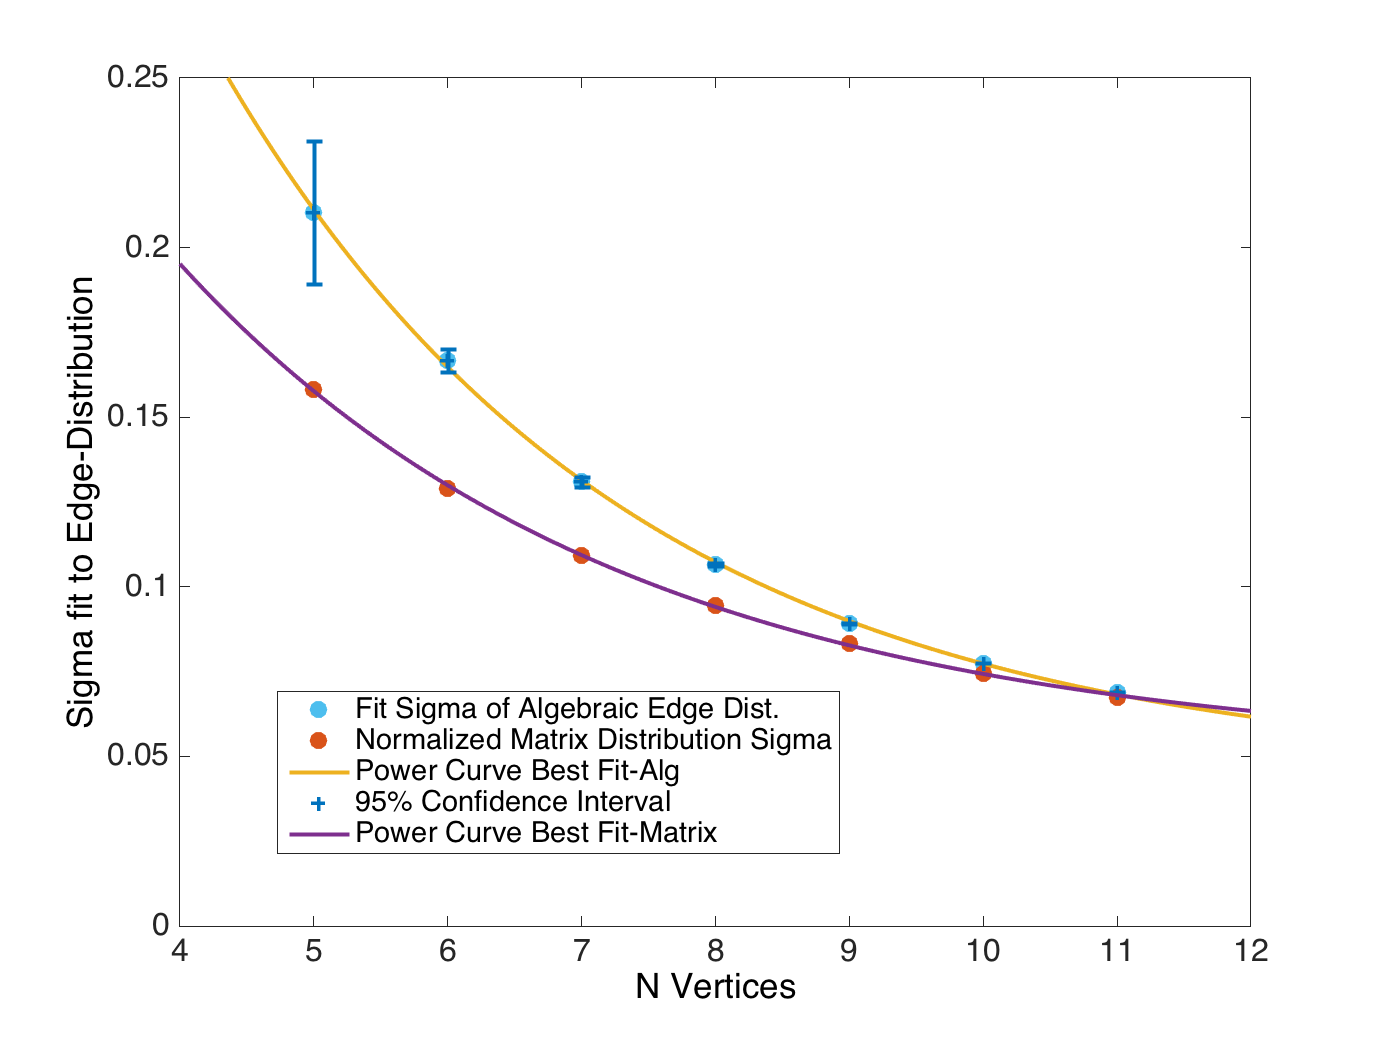
\includegraphics[width=\textwidth]{decreasingsigmawithbinom}
\label{fig:sigmaconvergence}
\end{figure}

Note that the values appear to shrink in their disparity, a remarkable observation, which gives us an idea of how the two sets/distributions differ with respect to the number of edges they produce as a function of $N$.
However, fitting exponential functions to each muddles the question: are they converging or intersecting and diverging again?
Note that even a convergence doesn't tell us about other properties of the sets of graphs.
Similarity in the distribution of the number of edges (or connectivity) does not equate distributional symmetry.
However, what we can see is that the Gilbert graph generator models the number of edges successfully for values of $N \approx 11$, and for larger values it may or may not  mirror this distribution.

%----------------------------------------------------------------------------------

\section{Specifically Disadvantaging Highly Automorphic Graphs}

Dominant models of random graph generation specifically preference graphs with fewer non-trivial automorphisms over graphs that have many automorphisms. 
This flaw is most glaring when discussing average or worst case running time over the `random' class of graphs.
Many algorithms make exciting claims about their performance on `random' graphs, but
we will show how theoretical and practical analysis of performance changes dramatically under different random graph generators.

\subsection{Two Quick Justifications}

To get an initial sense of this problem, we will first examine the relative probabilities of selecting a Co-Cycles graph from the set of graphs of size 10.
Since we know all 116 Co-Cycles graphs over 10 vertices, we can (without much computational effort) calculate the relative probabilities of generating a Co-Cycles graph under the standard (Gilbert) model and under the idealized model.
The results are not shocking, but a notable difference is apparent:
$$P(CoCycles(G) | G \in Gilbert) = \frac{\sum_{g \in CoCycles}^{116}M_{reps}(g)}{N Matrices} = \frac{260820000}{3.5184 \times 10^{13}} = 7.4130 \times 10^{-6}$$
$$P(CoCycles(G) | G \in Gilbert) = \frac{N CoCycles Graphs}{N Graphs} = \frac{116}{12005168} = 9.6625 \times 10^{-6}$$

Though these are not exorbitent differences, it should be noted that there is a difference of 23\%, meaning that by using a Gilbert random graph generator, you are 23\% less likely to observe a co-cycles graph as a result of generating one random graph than you would be via an idealized generator.
In this case, the difference between the generators is clearly appreciable, but not severely limiting.

As a second example, we will compare the most and least likely graphs to be observed under either random graph model.
In an idealized random graph generator, all graphs have equal probability of being selected.
Thus, the ratio of the most likely to least likely is exactly 1.

In a Gilbert random graph generator (abstracting over p, as discussed earlier), graphs that are fully automorphic (where the automorphism set contains all one-to-one mappings), are the least likely to occur.
One such graph is the fully connected graph, or the complete graph ($K_N$).
This is simply because the number of matrices which represent them is given by $M_{reps}$, and the probability of selecting a the complete graph is thus:
$$P(G = K_N | G \in Gilbert) =  \frac{M_{reps}(K_N)}{NMatrices} = \frac{N! / |Aut(K_N)|}{2^{.5N(N-1)}} = \frac{N! / N!}{2^{.5N(N-1)}} = \frac{1}{2^{.5N(N-1)}}$$
However, if we examine a graph with only the trivial automorphism ($G_{TA}$):
$$P(G = G_{TA} | G \in Gilbert) =  \frac{M_{reps}(G_{TA})}{NMatrices} = \frac{N! / |Aut(G_{TA})|}{2^{.5N(N-1)}} = \frac{N! / 1}{2^{.5N(N-1)}} = \frac{N!}{2^{.5N(N-1)}}$$
Thus, the ratio of these probabilities is always going to be $N!$.

These two examples give us a really important message: the difference between the Gilbert and Ideal models is frequently substantive, but its effects can be mild (as in the case of co-cycles graphs), or extreme (as in the case of selecting a perfectly automorphic graph).
What largely determines the degree of this distortion is the \emph{average number of automorphisms in the set that is being examined}. 
The larger this number, the more distortionary the Gilbert Model is when compared to the Idealized model.

\subsection{Theoretical Average Case Comparison}

Consider a standard canonical labeling algorithm.
This algorithm has two abstract components, one which correctly places vertexes into Similar Vertex Sets (SVS), and another which finds a canonical labeling given an accurate SVS partition.
If we take the first part of this algorithm as given, and assume that it can be computed in polynomial time (a reasonable assumption, as discussed in the section on SVS), then the running time of the algorithm is contingent upon the number of matrices we need to evaluate against some canonical property.
One common property for canonization is selecting the adjacency matrix which is the lexicographically smallest (or largest) representation of the graph.
It is reasonable to assume that the second half of the algorithm dominates the running time of the overall algorithm, as it is the piece that is inherently exponential based on the number of representations of the matrix.
Thus,  we can express the running time of the overall algorithm in terms of $O(|Aut(G)|)$, as this is the number of possible labelings we will have to examine to find our canonical one.

The selection of this simplified algorithm for analysis is not an accident: we have chosen it because the number of matrix representations ($M_{rep}(G)$) for a given graph $G$ is $\frac{N!}{|Aut(G)|}$.
Thus, if we are considering the average running time of this canonization algorithm ($\xoverline{T}_{Gilbert}$) over the set of all graph instances ($G_{inst} = G(A)$ for $A \in \{\{0,1\}^{N \times N}\}$) (i.e. using the standard models for random graph generation), we come to different conclusions if we consider the set of possible graphs $G_{inst}$, versus if we consider the set of all graphs as algebraic structural objects ($G_{alg}$).
$$\xoverline{T}_{Gilbert} = \frac{ \sum_{g \in G_{inst}} O(T(g))}{|G_{inst}|}$$
$$\xoverline{T}_{Gilbert} = \frac{ \sum_{g \in G_{alg}} O(T(g)) * M_{reps}(g)}{|G_{inst}|}$$
$$\xoverline{T}_{Gilbert} = \frac{ \sum_{g \in G_{alg}}  |Aut(g)| * \frac{N!}{|Aut(g)|}}{|G_{inst}|}$$
$$\xoverline{T}_{Gilbert} = \frac{ \sum_{g \in G_{alg}}  N!}{2^{.5(N^2 - N)}}$$
$$\xoverline{T}_{Gilbert} = \frac{ |G_{alg}| * N!}{2^{.5(N^2 - N)}}$$

This property might not look like it tells us much, but we can actually approximate what it looks like for different values of $N$, since we have the frist nineteen values of this sequence from OEIS sequence A000088.
This data is shown below.

However, if we attempted to select a graph from the set of all graphs of that size, we would find that: 
$$\xoverline{T}_{Ideal} = \frac{ \sum_{g \in G_{alg}}  O(T(g)) }{|G_{alg}|}$$
$$\xoverline{T}_{Ideal} = \frac{ \sum_{g \in G_{alg}}  |Aut(g)|}{|G_{alg}|}$$
$$\xoverline{T}_{Ideal} = \text{Average Number of Automorphisms over Graphs}$$

Some sample numbers to give you the scale of these disparities is given below.

The takeaway here is that specifically disadvantaging a class of graphs (namely highly automorphic graphs) warps our analysis of running time in a substantive way, not only for fringe algorithms, but for well studied algorithms too.
We can show this through the theoretical proof as shown above, but we can also show it through data describing actual algorithm performance.

\subsection{Practical Average Case Comparison}

The NAUTY package is one of the quickest algorithms for canonical labeling.
Though its performance is weaker on some graphs (like the Miyazaki, for example), in general, its canonical labeling algorithm is widely regarded and frequently used.

I ran the NAUTY canonization algorithm on batches of graphs with different numbers of edges, to get a sense for how the running time changes when we change the way that we randomly generate the graphs.
Shown in figure \ref{fig:nautyperformance10} is how the NAUTY algorithm performs against varrying values of $p$ for $N=10$.
Each was run thirty times, and the margin of error (as a 95\% Confidence Interval) is shown around each of the estimates.

\begin{figure}[h]
\caption{}
\centering
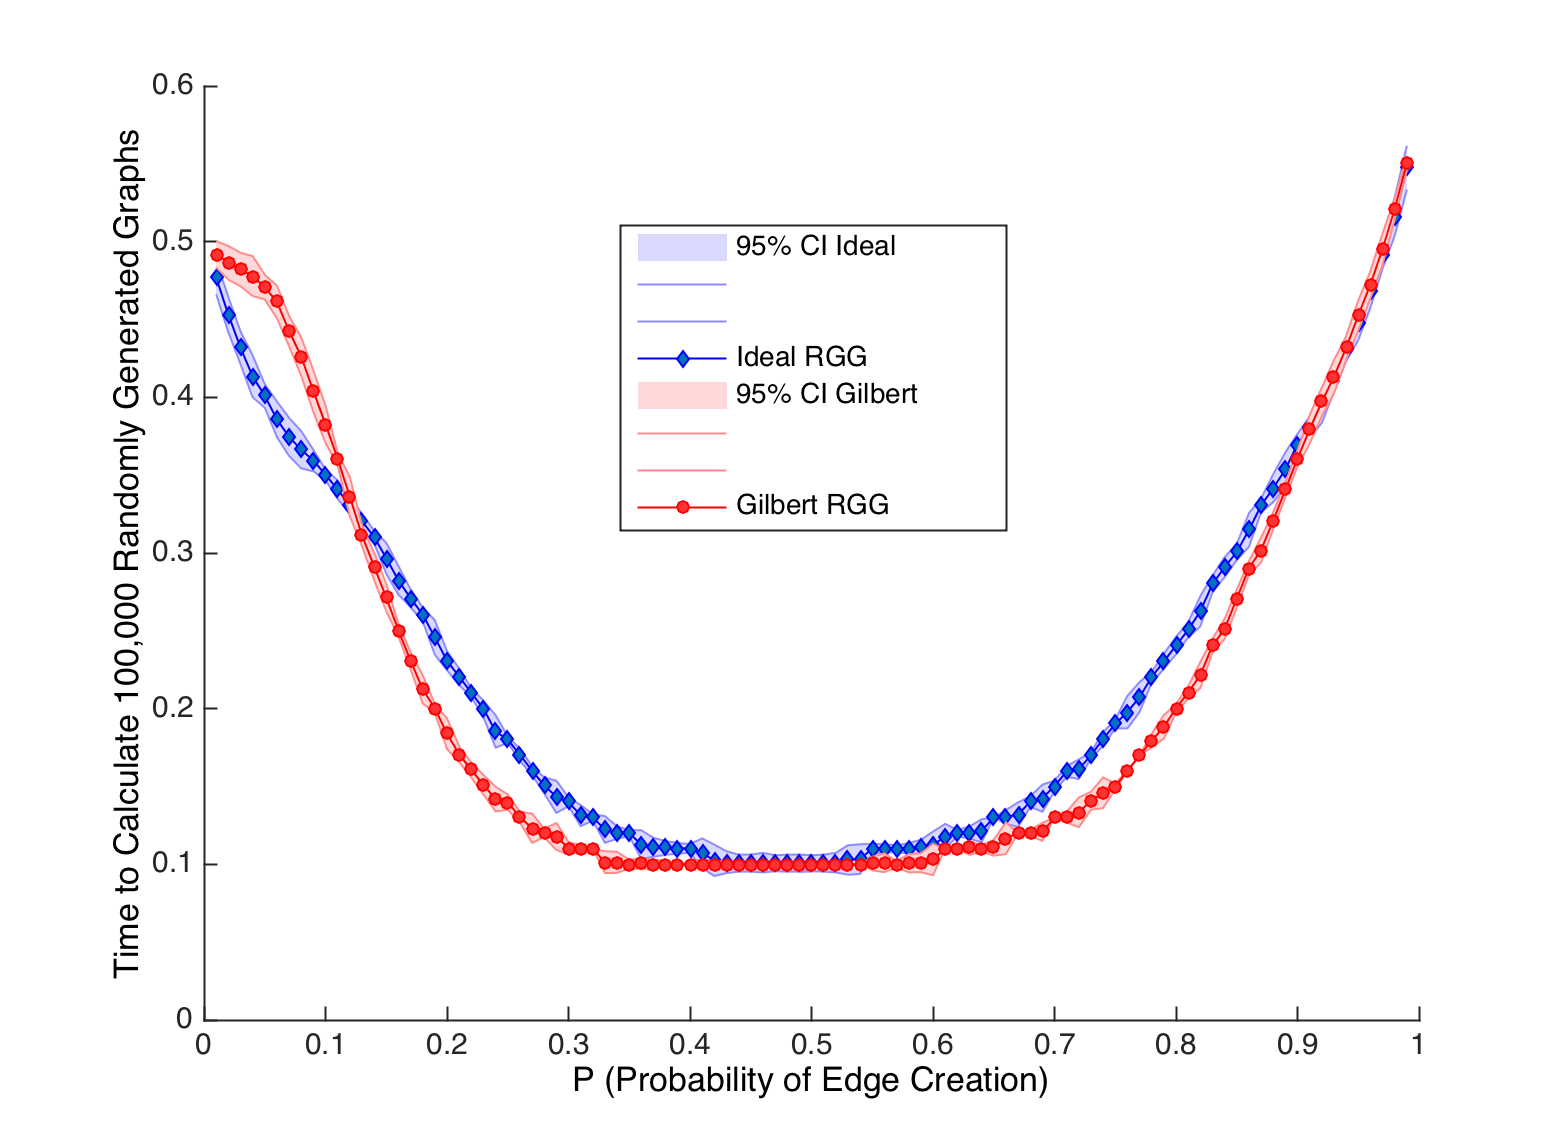
\includegraphics[width=\textwidth]{nautyperformance}
\label{fig:nautyperformance10}
\end{figure}

We can see from this figures that not only does NAUTY have slower performance on `Idealized' random graphs, but there are crossover effects.
The integral between these curves works out to about a 10\% increase in running time between the Gilbert RGG and Idealized RGG.

Both in theory and in practice, distinguishing between 'random graph' and `random graph instance' has significant implications.
It is very possible that misuse of the Gilbert model has understated the true average and worst case time complexity for a number of algorithms, including the NAUTY algorithm.

\subsection{Should We Never Use the Gilbert Model?}

The short answer to this question is no, the Gilbert model is remains relevant (even dominant) even when we embrace these flaws.
The primary argument for the Gilbert model is not its application to questions of theory, \emph{but questions of practice and natural occurrence}.
Most applications of graph theory to world problems are based around structures that are naturally arising, without centralized planing or design.
It is much more likely that some graph that is found in the world will be non-automorphic than have some kind of inherent and difficult to describe complexity.
This is because if we look at graph building as a process (in the Gilbert model), or as a probabilistic construction (in the Erdos-Reyni model), then some outcomes are more likely than others.
This is well in line with the assumptions of the models: that graph instances are suitable placeholders for their graphs.

Rather, what we have been criticizing is the \emph{application} of the Gilbert model to questions about theoretical algorithmic complexity.
In graph theory, we hold a meaningful distinction between graphs and graph instances, a distinction only made at the theoretical level.
It is thus inappropriate to use a model which ignores this distinction, and ignores it in such a way as to specifically disadvantage certain classes of graphs.
This allows theoretical arguments about graph algorithms to underweight what we consider `hard' cases, and overweight what we would generally consider `easy' cases.

This distinction is important.
In practice, graphs that arise in the world are likely to be selected randomly from the set of graph instances.
However, in graph theory, where we consider isomorphic graph instances to be fundamentally equivalent, the assumptions of the Gilbert model are antithetical to other assumptions of graph theoretic research.

\section{Measuring and Comparing Random Graph Models}

Our mandate suddenly becomes: `well, what can we do which is better?'
Establishing an intuition to answer this question requires us first to understand what we would think of as `ideal', and see if we can approach that model.

\subsection{An Ideal Random Graph Model}
To allow our comparisons to be explicit, we will use the same nomenclature to describe an idealized generator as we do with the Gilbert model, so that they are directly comparable.
Thus, our ideal random graph model will take two input parameters, $N$ and $p$, where $p$ describes the probability of getting any given edge existing.
Note that this explicitly breaks from the idea of edge independence that is assumed in the Gilbert model.
Rather, we are assuming that the probability of any given edge existing is $p$ if we have no knowledge about the rest of the graph.
We will define our `Ideal' generator as one which first selects a number of edges $M$ from the binomial distribution with $E_{Max}$ trials and trial success probability $p$.
After selecting $M$ as an observation from this random distribution, we will select a graph from the set of all graphs of $N$ vertices and $M$ edges with uniform probability.
To accomplish this task, we will enumerate all graphs of that size, and select from that fully defined set.

The flaw in this scheme is obvious.
Our `Ideal' generator is only possible by this methodology so long as you can enumerate all graphs of a given size.
There are 24637809253125004524383007491432768 non-isomorphic graphs over 19 vertices, so this is not remotely sustainable methodology for a random generator.
If we cannot rely on an ideal graph generator, are we doomed to stick with the Gilbert model?
Or, could we create a model that is better than the Gilbert model (closer to our ideal), while being computationally reasonable?

\subsection{An Equivalent Ideal Random Graph Model}

Another way to view our equivalent random graph model is as a overlaid construction on top of a standard, Gilbert, random graph model.
Since we know that the Gilbert random graph model produces a graph with a probability proportional to its number of automorphisms, we can actually create a random graph generator which is equivalent to our idealized model by systematically throwing out graphs with probability inverse to their probability of showing up.
The algorithm which generates to this model is not guaranteed to halt, but does simulate our idealized random graph generator, even over large values of $N$.

\begin{lstlisting}[frame=single]
while true:
	g = gilbertRandomGraph(N, p)
	na = |Aut(g)|
	p = Math.rand(0, 1)
	if (p < (na / N!))
		return g
\end{lstlisting}

Here we find a gilbert random graph, and calculate the number of automorphisms that it has.
That gives us knowledge of how many times we would expect it to occur in a sample of $2^{E_{max}}$ random graph instances, namely $N! / na$ times.
Thus, we weight any randomly observed random graph instance by the inverse of this value.
This equalizes the probability of getting any graph, regardless of its number of automorphisms.

This methodology is, unfortunately, equally unsustainable.
This is an example of a geometric process, where we will have to go a certain number of trials before finding a success and stopping. 
The probability of a success on any given trial is $p = \frac{|G_{alg}|}{|G_{inst}|}$, which approximates the $p = fact^{-1}(N) = \frac{1}{N!}$ growth function.
Thus, for even a small number of vertices, the expected number of trials that need to be generated before a success is found is very large, as it is given by $1/p = N!$. 
For example, if $N=10$, we would expect to have to examine 3.6 million graphs before finding one which is returned successfully.

This too, is not a sustainable methodology for random graph generation.

\subsection{Establishing a Methodology for Random Graph Generator Evaluation}

So what can we do that is better?
Answering that question required some really deliberate thought.
I knew lots about what I didn't want to do:
\begin{itemize}
\item{I didn't want to use subjective measures to support one random graph generator over another.}
\item{I didn't want to write generators and then use collected data to support them.}
\item{I didn't want to focus in on singular ways of looking at the quality of the graphs that I generated.}
\item{I didn't want to allow my own intellect and lack of creativity be a limiting step on the way to a better generator.}
The process that I decided on attempted to address all of these concerns, and was designed to avoid the pitfalls of bad computer science: overfitting, statistic selection, and rigidity.
\end{itemize}

I decided on a wide portfolio of statistics each of which is calculated over a sets of graphs.
These statistics are inherently heuristic, but each attempts to capture some property of the graphs that are generated, or some property of how the set looks as a whole.
Each of the statistics I decided on is meant to describe some property of a set of graphs, but it does not establish an `idealized' or theoretical value for that statistic.
Though for several of these metrics we know how to express the ideal/expected probability, that is not always the case (or not always known to be the case0.
These metrics serve as a way for us to identify and name ways that random graph generators fail us, and challenge us to do better, to compare a proposed solution to an ideal or standard solution in quantifiable and concrete terms.

The set metrics is described in the next section, and they vary in computational complexity and broad descriptiveness.
I set up a (pardon the brag) BEAUTIFUL system for calculating these statistics over arbitrary datasets.
I created an idealized random generator (as described above), and a Gilbert random generator, and verified the accuracy of the results produced through this computational system over the initial results from each.

Most importantly, I set up these metrics, this system, and the baseline Gilbert/Ideal metric values before I wrote a line of code which randomly generated graphs.
This is really important to me, because it frees the results of this work from the publication and statistic selection bias that plagues research everywhere.

\subsection{Graph Set Metrics}
Below are the metrics that I compared across graph sets generated by different random graph generation procedures.
Though I calculated some more statistics for personal use and discovery, the ones included below are the `single result' statistics.
Others were distributional properties that were not easily captured and compared (except through distributional goodness of fit tests, which only give us an idea of alikeness, not of directed difference).
The reliance on singular metrics as a means of comparison allows us to evaluate systems of random graph generation automatically, and come up with similarity tests that are divorced from our intuition and hypotheses.

Described below are each of the metrics that are calculated over every set of random graphs that were generated.
Each is labeled a statistic (implying a singular value used to judge the generator) or a distribution (connoting that it was not used in the systematized evaluation of generators).
Each is listed under its acronym, which can be found throughout my code and tests. 

\subsection{Graph Set Metric Reference, Coding and Description}

\begin{itemize}

\item{ADIAM - Set Statistic - Average Graph Diameter - Take the diameter of each graph, and average over all graphs in the set}
\item{ADSM - Set Statistic - Average Degree Sequence Mean - take the mean of degree sequence of each graph, and average that across all graphs}
\item{ADSMD - Set Statistic - Average Degree Sequence Median - take the median of the degree sequence of each graph, then average that across all graphs}
\item{ADSMN - Set Statistic - Average Degree Sequence Minimum - take the degree of the least connected node in each graph, then average that across all graphs}
\item{ADSMX - Set Statistic - Average Degree Sequence Maximum - take the degree of the most connected node in each graph, then average that across all graphs}
\item{ADSR - Set Statistic - Average Degree Sequence Range  (i.e. Find the difference in degree between the most and least connected node, and average over all graphs in the set}
\item{ADSV - Set Statistic - Average Degree Sequence Variance - take the variance of the degree sequence of the graph, then average across all graphs}
\item{ALNA - Set Statistic - Average of the Logarithm of the Number of Automorphisms - Find the number of automorphisms that each graph has within the set, take the logarithm of each, then average across the logged results}
\item{ANA - Set Statistic - Average Number of Automorphisms - find the number of automorphisms for each graph, then average that across the set}
\item{ANCC - Set Statistic - Average Number of Connected Components - take the number of connected components of each graph in the set, then average across all of them}
\item{ANQUAD - Set Statistic - Average Number of Quadrilaterals - The Average number of non-trivial (non-edge repeating) quadrilaterals across all graph instances within the graph set.}
\item{ANR - Set Statistic - Average Number of Repeats - The average graph, when selected from the set in question, will have this expected number of equivalent instances in the set}
\item{ANTRI - Set Statistic - Average Number of Triangles - The Average number of triangles across all graph instances within the graph set.}
\item{CP - Subset - Co-Cycles Graphs - The intersection between the set of all $V=10$ co-cycles graphs and the given set}
\item{DIAMV - Set Statistic - Variance in the Diameter of Graphs - calculate the diameter of each graph, and calculate the variance of the set as a whole}
\item{DSMDV - Set Statistic - Degree Sequence Median Variance - Take the median degree of each graph, and calculate the variance over all graphs in the set}
\item{DSMNV - Set Statistic - Degree Sequence Minimum Variance - Take the minimum degree of each graph, and calculate the variance over all graphs in the set}
\item{DSMV - Set Statistic - Degree Sequence Mean Variance - Take the mean degree of each graph, and calculate the variance over all graphs in the set}
\item{DSMXV - Set Statistic - Degree Sequence Maximum Variance - Take the maximum degree of each graph, and calculate the variance over all graphs in the set}
\item{DSVV - Set Statistic - Degree Sequence Variance Variance - Take the variance of the degree sequence of each graph, and calculate the variance over all graphs in the set}
\item{FC - Set Property - Frequency Count - The number of isomorphic graph instances associated with each one of the graphs in the set}
\item{FFC - Set Distribution Counts - Frequency Count Counts - The counts that correspond to FFVs, the frequency with which graphs show up in our random set}
\item{FFV - Set Distribution Bins - Frequency Count Bins - The discrete values for which there exist graphs in our set that poses that number of instances in the set, this is really just a bin count for FC}
\item{MLNA - Set Statistic - Median of the Logarithm of the Number of Automorphisms - Find the number of automorphisms that each graph has within the set, take the logarithm of each, then find the median across the logged results}
\item{MNR - Set Statistic - Maximum Number of Repeats - The graph in the set that was selected the most times was selected this many times}
\item{NA - Graph Statistic - Number of Automorphisms - Counts the number of automorphisms that a graph has by finding the number of unique matrices that describe a graph}
\item{NAB - Set Distribution Bins - Number of Automorphisms Bins - The unique values of NA, to provide histogram alongside NAC}
\item{NAC - Set Distribution Counts - Number of Automorphisms Counts - The counts of the NAB, as in a histogram}
\item{NCCV - Set Statistic - Variance in the Number of Connected Components - take the number of connected components of each graph in the set, then take the variance of the set}
\item{NCP - Set Statistic - Number of Co-Cycles graphs - Same as Co-cycles graphs, this only applies to graphs of size 10 and larger, counts the number of Co-Cycles graphs (which tend to be highly automorphic) in the overall set of graphs}
\item{NE - Set Statistic - Number of Edges - the average number of edges in the graph set. This should be the same across generators, as we are specifying $p$, and asking for a large sample size}
\item{NR - Set Statistic - Number of Regular Graphs - the number of regular graphs in the graphset}
\item{NUG - Set Statistic - Number of Unique Graphs - The proportion of graphs within the set that are only generated once}
\item{ODSPL - Set Statistic - Overall Degree Sequence Poisson Distribution Lambda  - Find the set of all of the degrees of all of the graph, then fit a poisson distribution to this distribution. Report the lambda that defines this poisson distribution}
\item{PCONN - Set Statistic - Probability of Connectivity - take the number of fully connected graphs, and divide by the total number of graphs in the set}
\item{PDL - Set Statistic - Poisson Distribution Lambda - Take the distribution of the number of times that each graph is represented by an instance within a graph set, and set this distribution fit to a poisson distribution, reporting its lambda}
\item{PQRA - Set Statistic - Percentage Quazi-Regular A - Percentage of graphs where the degree sequence range is less than or equal to 1}
\item{PQRB - Set Statistic - Percentage Quazi-Regular B - Percentage of graphs where the degree sequence range is less than or equal to 2}
\item{PQRC - Set Statistic - Percentage Quazi-Regular C - Percentage of graphs where the degree sequence range is less than or equal to $sqrt(N)$}
\item{PTRIL - Set Statistic - Probability Triangle-less - the Probability that a graph instance selected randomly from the graph set is triangle-less.}
\item{SQNR - Set Statistic - Sum of Squared Number of Repeats - A measure of how dispersed the distribution is, calculated as $FFC \dot (FFV^2) / nGraphs$}
\item{UG - Set Property - Unique Graphs - The canonical form of all of the graph set's graphs, with duplicates removed (if they existed)}
\item{VLNA - Set Statistic - Variance of the Logarithm of the Number of Automorphisms - Find the number of automorphisms that each graph has within the set, take the logarithm of each, then find the variance of the logged results}
\end{itemize}

\subsection{Establishing Baselines for Graph Set Metrics}

Once we set up these metrics, we need to find a way to systematically compare them within our desired context: building a random graph generator which models an idealized random graph generator.
To do this, I established baseline understandings for each one of the metrics, over a problem `domain':
\begin{itemize}
\item{Number of Graphs - I decided to operate over sets of 1000 graphs.  It allowed us to get reasonable numbers for standard deviations and not use an excess of CPU time}
\item{Number of Vertices - I baselined the metrics over graphs of size 4 to size 10.  This allowed us to see what the metrics looked like on an overrepresented graph set, and on a sample set.}
\item{Probability of Edges - I used p from the set $[.1, .2, .3, .4, .5, .6, .7, .8, .9]$. I figured that focusing on sparse, dense or intermediate graphs might introduce biases that I hadn't accounted for, so I decided for the most generic set possible.}
\item{Number of Trials - For each one of these baseline scenarios, I performed 30 trials}
\end{itemize}

Thus, in the end, there were $2 \times 9 \times 7 \times 30 = 2780$ sets of 1000 graphs that were used to create our baseline metrics.

For each one of the statistics we calculated the mean and standard deviation of the sampled metrics over both algorithms.
That resulted in two sample means and sample standard deviations, for the ideal and gilbert graph models: $\xoverline{x_I}, \xoverline{x_G}, s_I$ and $s_G$. 
Using these values, I came up with a simple and intuitive way to measure a new random graph generator, given its value for $\xoverline{x_N}$ and $s_N$ and the number of samples that were used to compute each, $n_N$.
This methodology compares the t values in two tests of significance for two unknown means and unknown standard deviations.
In a test of unequal unknown means and standard deviations, the slightly modified t-statistic is given by:
$$T(A, B) = T(\xoverline{x_A}, \xoverline{x_B}, s_A, s_B, n_A, n_B) = \frac{|\xoverline{x_A} - \xoverline{x_B}|}{\sqrt{(s_A^2 / n_A + s_B^2 / n_B}} $$
And our scoring mechanism for a metric and generator is given by:
$$ \text{Score for Metric M} = -1 * \text{min} \bigg[ \ln \Big( \frac{T_M(I, N)}{T_M(I, G)} + e^{-10} \Big), 10 \bigg] $$
Lets break down this scoring mechanism:
\begin{itemize}
\item{First off, $T_M(A, B)$ is strictly greater than or equal to zero (and all of our metrics have non-zero $T_M(I, G)$ values), thus the fraction in the logarithm is defined and in the range $[0, \infty)$. When we add $e^{-10}$, we shift that range up to $[e^{-10}, \infty)$, meaning that the logarithm's value will be bounded between $[-10, \infty)$ }
\item{Next, we take the minimum of this score and 10, to bound the individual score between $[-10, 10]$.}
\item{Finally, we invert the values with a -1, so that a score of -10 corresponds to a metric where the new random graph generator performs incredibly poorly, while 10 corresponds to a metric where the new random graph generator is indistinguishable from ideal (with respect to the differences setup by the baselines).}
\item{The resulting metric has the helpful property that the baseline metric is at (or ever so slightly below) 0, so that a score of 0 marks an equivalence in quality to the Gilbert random generator.}
\end{itemize}
Once we calculate individual metrics, we can calculate the score for a generator as the sum over the number of metrics that are calculated for it, which includes multiple values of p and n:
$$ \text{Score for Generator} = \frac{1}{N_{Metrics}} \times \sum_m^{Metrics} Score_m $$
in this metric, higher scores are better and a score of 0 corresponds to a generator that is exactly as bad as the Gilbert Generator.

This is a good mechanism because it scores a value on a metric based on how close it is to the ideal mean, but also compares any deviancy to the deviancy observed between the ideal and standard (Gilbert) generators.

\subsection{Finding Data on Graph Set Metrics and Scores}

The baselines for the graph set metrics are all stored in one file for convenience (Thesis/Matlab/Alternative Generator/Data/baselineMetrics.mat).
As mentioned above, they are for the tenth-probabilities, over graphs of size 4 to 10.
The baselined metrics were constructed using thirty random trials, each containing 1000 random graphs.
In the baseline file, the mean, standard deviation and number of samples is given.

An appendix to this thesis lists the graph set baselined metrics, along with their associated uncertainties, for all values of $N$ and $p$.
Since there were 7 tested values of $N$, and 9 tested values of $p$, and 35 metrics, over two different generators for random graphs, there are a total of approximately 4,000 component statistics in this baseline file.

\subsection{Examining the Difference between Gilbert and Ideal Baselines}

The differences between the Gilbert random graph generator and the Idealized generator are on display in the visual examination of the metrics described above.
To see the full range of differences, and the full set of charts that were generated to supply some of these examples, please check out my code on github.
These files in particular are stored at /Thesis/Matlab/alternative generator/analysis.

In this section, we will summarize the broad tendencies (and larger deviations) that we see between the two models.
There are six different categories that I placed each of the metrics within, describing six different patterns of difference.
The graphs used for this section should be taken with a grain of salt: in our baselines, we perform 30x the number of trials that generated these graphs, so they certainly are prone to more vertical uncertainty.
However, we have graphed many more values of $p$, so these graphs can better show how the baselines change across values of $p$, not only see their absolute differences.

\subsection*{Identical - ADSMD, ADSMN, ANQUAD, DSMV, NE, ODSPL} 
Some of the metrics were indistinguishable between the two random graph generators.
Approximately six of the thirty-five metrics behaved indistinguishably between the Gilbert and Idealized random graph generators.
An example is shown in figure \ref{fig:anquad10} below, which describes the number of quadrilaterals in a graph set for various values of $p$ (the graphs were all of size 10, and there were 1000 of them represented by each dot).

\begin{figure}[h]
\caption{}
\centering
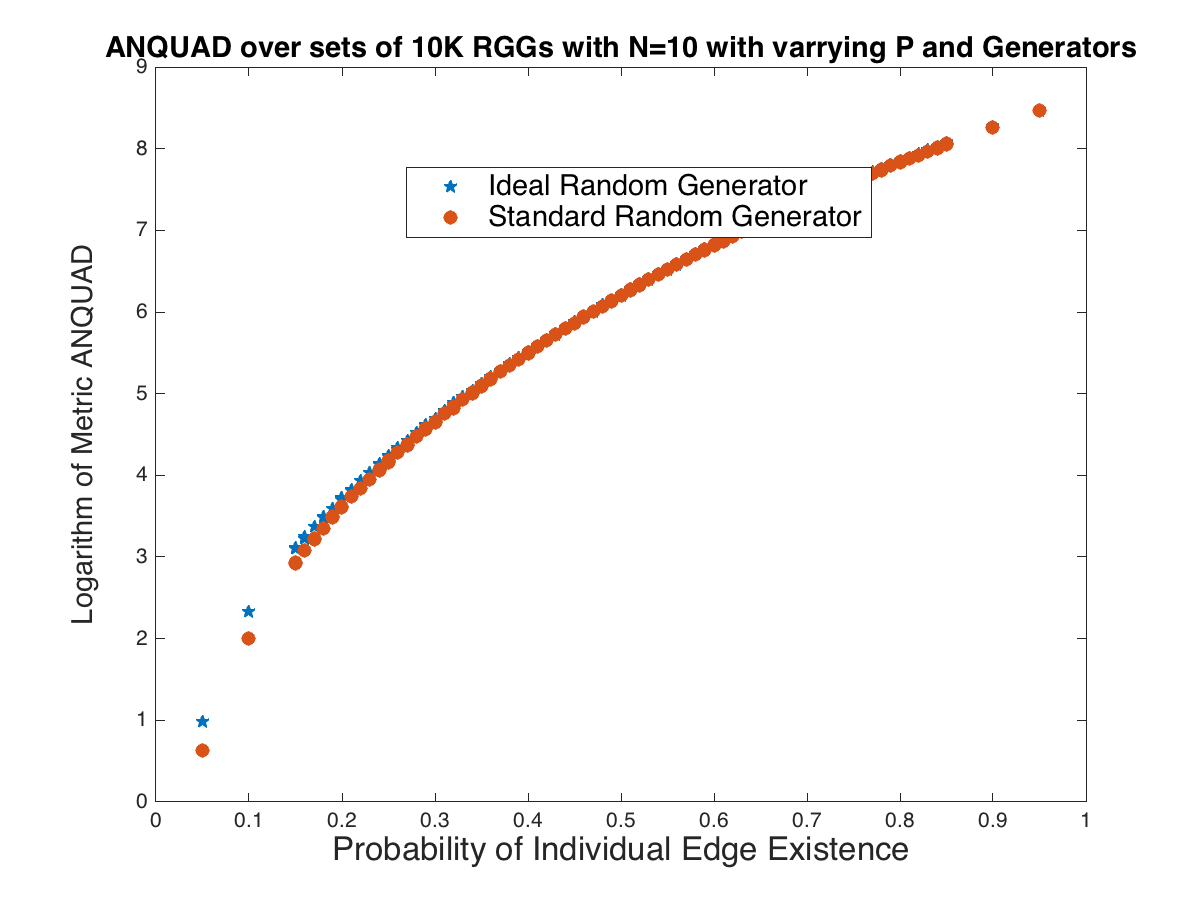
\includegraphics[width=\textwidth]{ANQUAD-10}
\label{fig:anquad10}
\end{figure}

\subsection*{Height Different - ADIAM, ADSMX, ANA, ANCC, ANR, ANTRI, DIAMV, MLNA, NCCV, NUG, PCONN, PDL, PQRA, PQRB, PQRC, SQNR} 
Many of the metrics had the same broad patterns in the way that they changed with respect to $N$ and $p$, but had slightly different heights/inflectuations.
The majority of graph metrics were in this category.
An example shown in figure \ref{fig:sqnr7} shows a metric which rises with duplicates (SQNR) over seven vertices.
Note that though the patterns are the same over the two methodologies, the results are hight separated.

\begin{figure}[h]
\caption{}
\centering
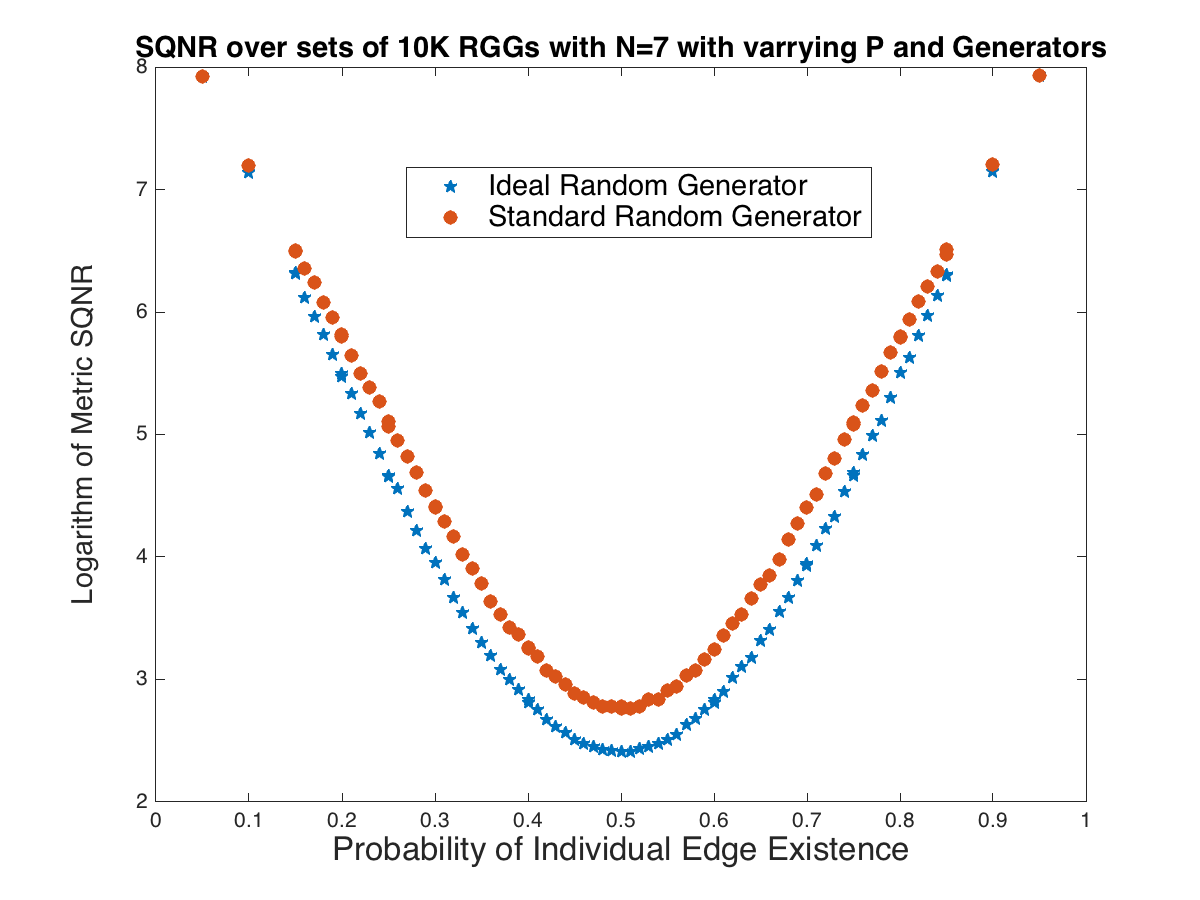
\includegraphics[width=\textwidth]{SQNR-7}
\label{fig:sqnr7}
\end{figure}

\subsection*{Not Enough Data - NCP}
For one metric, there was consistently not enough data to calculate it or any comparison between two random graph generators.
It shouldn't come as a surprise that that metric is NCP, the number of Co-Paths (or Co-Cycles) graphs in the graph set. 
Since there was consistently not enough data to establish a baseline, you will find that most of the time NCP is zeroed out, not by some choice of mine, but because of the way I have set up my scoring mechanism.

\subsection*{Crossover - ADSR, ADSV, NCCV, PTRIL, VLNA}

For five metrics, there was even more of a difference than height alone.
In these graphs, the two curves intersect/cross over so that a metric might be better on one range of $P$ and worse on a different range.
This significantly complicates the way we are able to do optimization to improve upon our graph metric scores. 
With most of the height different variables, clearly we are going to be able to create RGGs which can better mimic a height shift than fundamentally reexamining the nature of the curve.

Two examples are given below, one describes the variance in the diameter of graphs chosen (figure \ref{fig:diamv5}), and the other shows the variation in the logarithm of the number of automorphisms of each graph in the set (\ref{fig:vlna6}).

\begin{figure}[h]
\caption{}
\centering
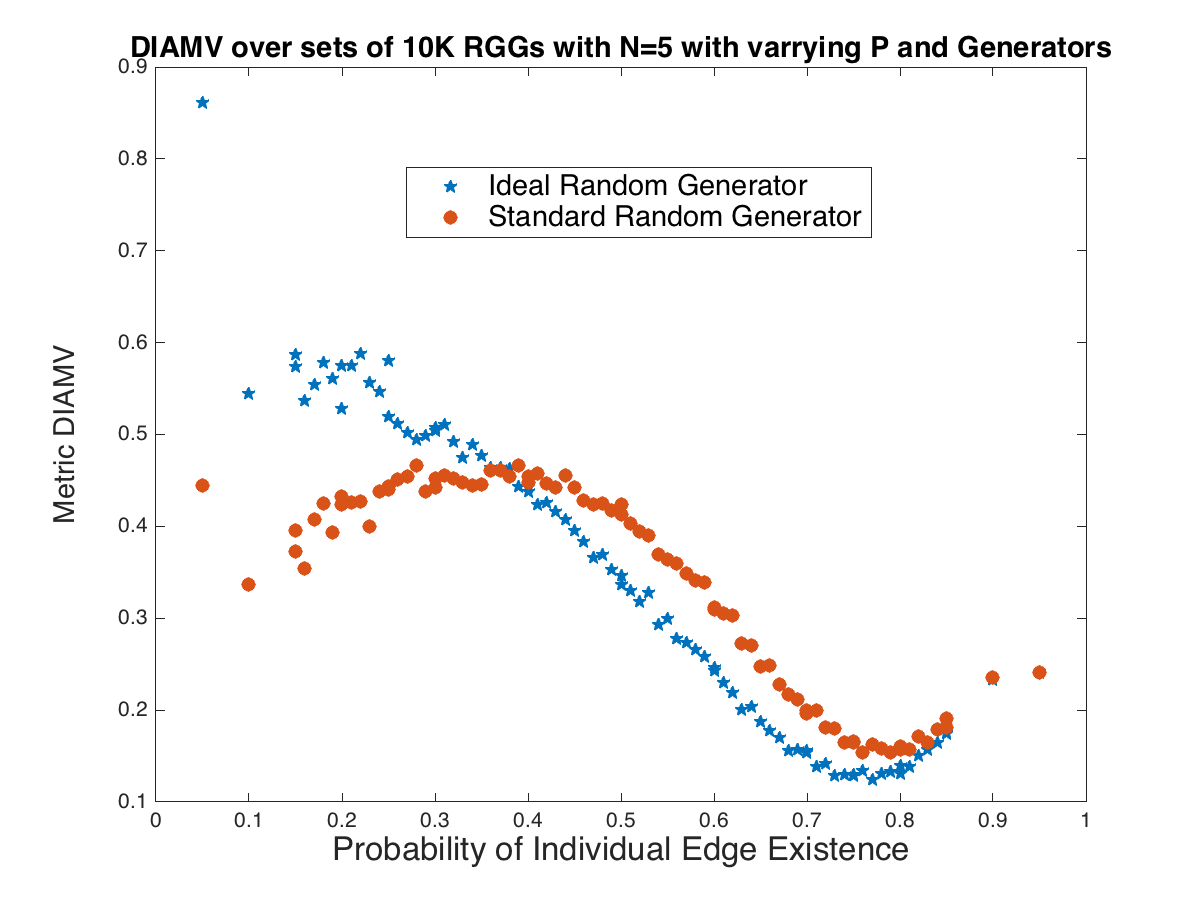
\includegraphics[width=\textwidth]{DIAMV-5}
\label{fig:diamv5}
\end{figure}

\begin{figure}[h]
\caption{}
\centering
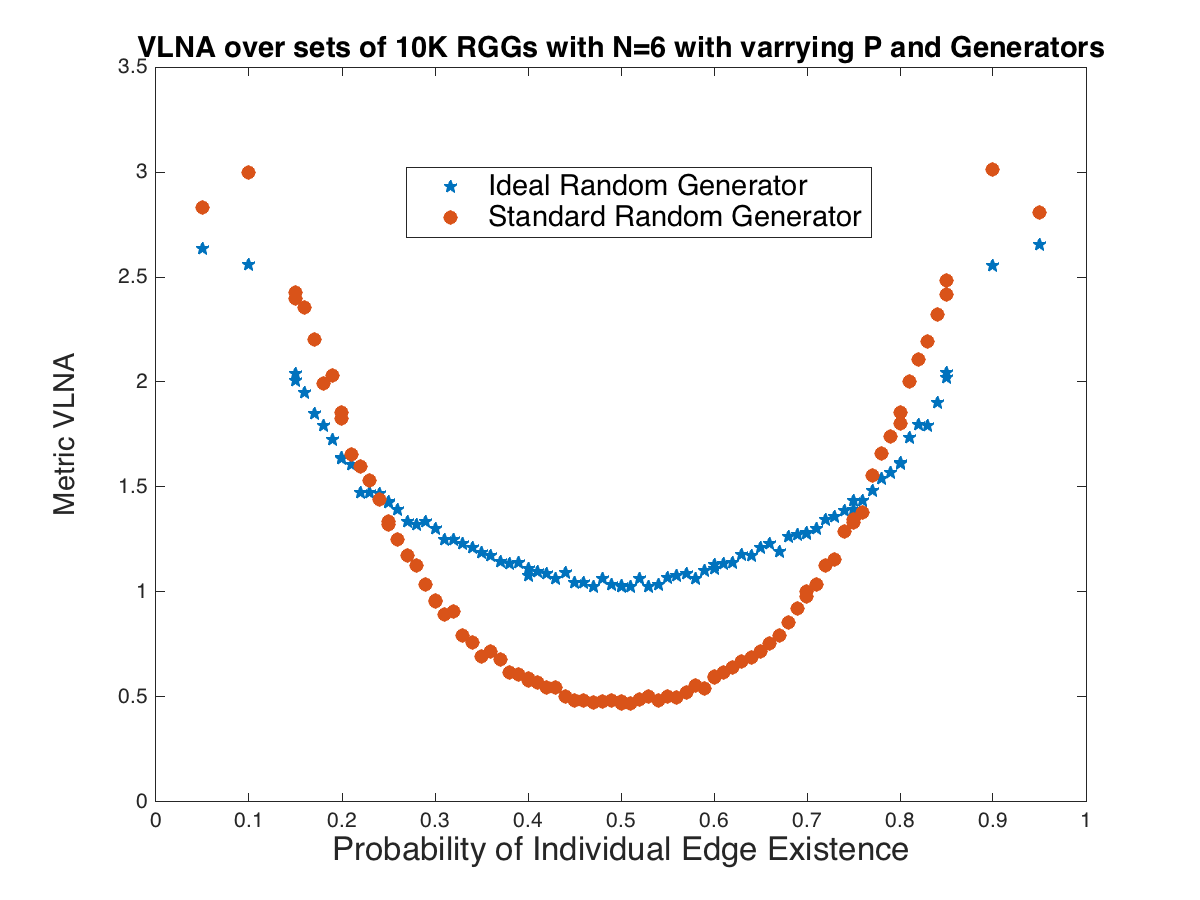
\includegraphics[width=\textwidth]{VLNA-6}
\label{fig:vlna6}
\end{figure}

\subsection*{Shape Different - ALNA, DIAMV, DSMDV, DSMNV, DSMXV, DSVV, MNR, NR}
Finally, many metrics simply displayed different shapes across different ranges of $p$.
Many of these metrics are variance metrics, possibly alluding to the way that graph sets as a whole are either varied or homogenous on each metric.
The two figures displayed show the degree sequence maximum (figure \ref{fig:dsmxv10}), and the average diameter of graphs in the set (figure \ref{fig:adiam9}).
We should remember that these are not trivial differences, and I think that the graphs really speak to that.

\begin{figure}[h]
\caption{}
\centering
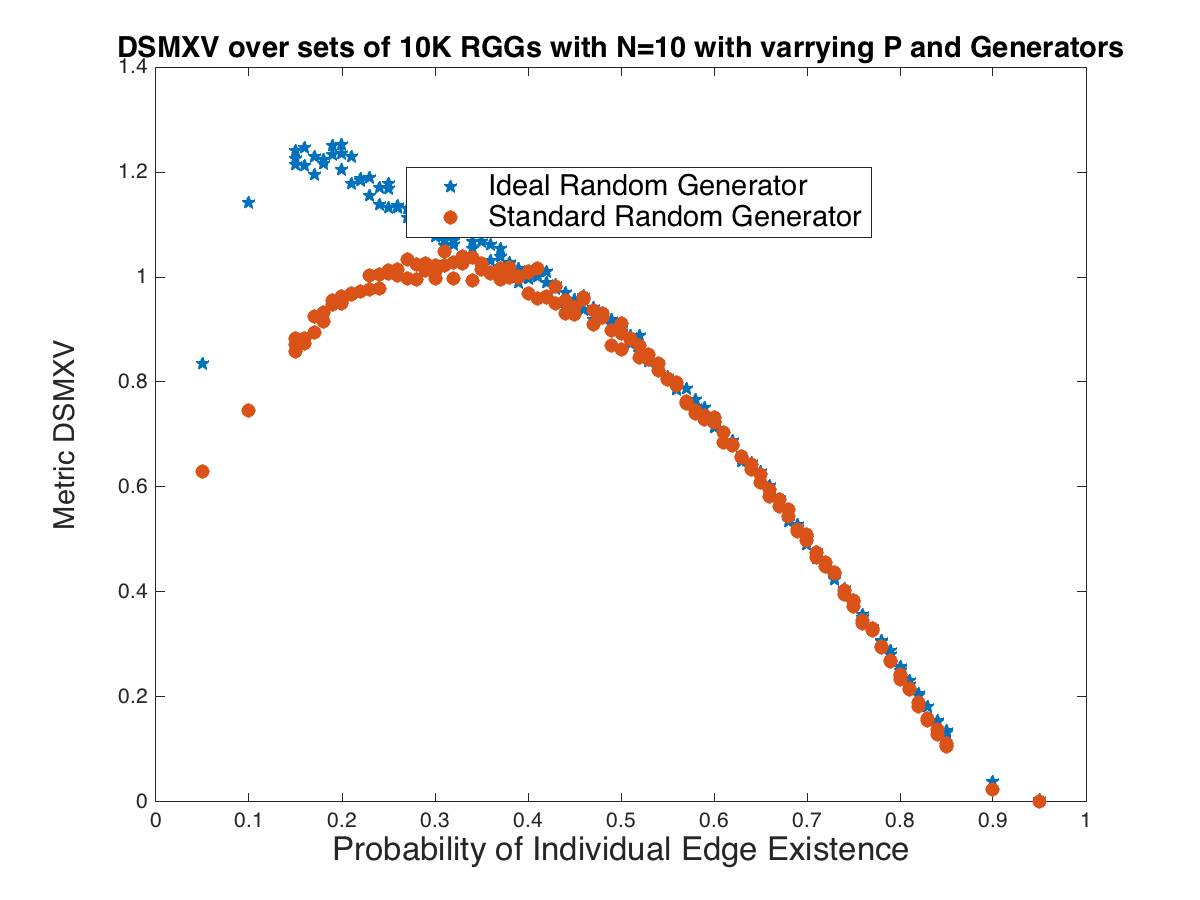
\includegraphics[width=\textwidth]{DSMXV-10}
\label{fig:dsmxv10}
\end{figure}

\begin{figure}[h]
\caption{}
\centering
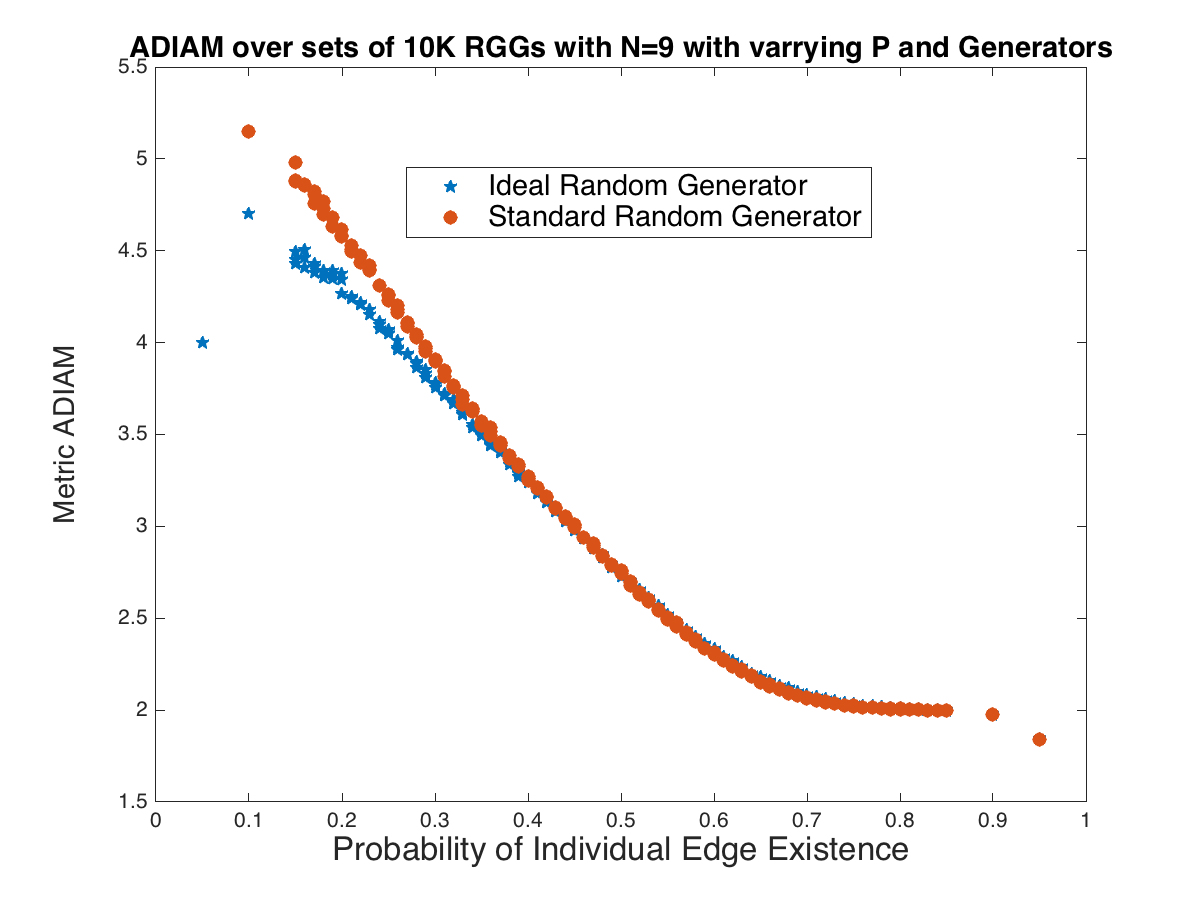
\includegraphics[width=\textwidth]{ADIAM-9}
\label{fig:adiam9}
\end{figure}

\section{Alternative Ideas for Random Graph Modeling and Creation}

Now that we have a mechanism for quantifiably adjudicating the quality of a proposed random graph generator, we are tasked with creating different ideas for random graph generation and evaluating them on this basis.
Discussed below are each of the algorithms that I built for Random Graph Generation and Processing.
They are not presented in any particular order.
Each is prefixed by the string that it is represented as/by throughout the code.

\subsection{MinusOne - A Weighted Automorphic Subgraph Generator}

MinusOne has a simple methodology.
If you are generating a graph with $N$ vertices and with probability of edge creation $p$, start by creating a graph $H$ of size $N+1$ via the gilbert model.
Then, generate all $N+1$ of $H$'s single vertex deleted subgraphs, store each in a set we will call $VD(H)$.
Lets define an automorphic metric $AM$ which is defined by the following formula, finding the QSVSes, and take the product of the factorial of their sizes.
$$AM(g) = \prod_{i \;\in \;QSVSes(g)} |QSVS_i|$$
Finally, over each member of the set $g \in VD(H)$ calculate the automorphic metric, and select that graph with the probability:
$$P(g | H) = \frac{AM(g)}{\sum_{h_i}^{VD(H)} AM(h_i)}$$

\subsection{MinusOneA - Less Automorphic Version of MinusOne}

MinusOneA has a methodology with closely matches that of MinusOne.
The only difference is the automorphic metric function, which is the logarithm of the one proposed above (plus a constant factor).
$$AM(g) = 1 + \log_2 \Big[{\prod_{i \;\in \;QSVSes(g)} |QSVS_i|} \Big]$$

\subsection{MinusOneB - Interspersing Some Gilbert Random Graphs}

MinusOneC has an identical methodology with closely matches that of MinusOne, with one caveat.
With a probability selected based on $p$, the algorithm chooses between picking a graph from a MinusOne distribution and a Gilbert distribution:
\[ MinusOneB(n, p) = \begin{cases} 
      Gilbert(n, p) & \text{if $rand < .5 * (p) * (1-p)$} \\
      MinusOne(n, p) & \text{otherwise} \\
   \end{cases}
\]

\subsection{MinusOneC - Less Automorphic Version of MinusOne}

MinusOneC has a methodology with closely matches that of MinusOne.
The only difference is the automorphic metric function, which is the square root of the one proposed above.
$$AM(g) = \sqrt{\prod_{i \;\in \;QSVSes(g)} |QSVS_i|}$$

\subsection{BuildingA - An Iterative Graph Generator}

Building Algorithms are processes by which edges are added individually to a matrix (given a `probability matrix'), and then a new probability matrix is generated from the current iteration of the formative graph.

\begin{lstlisting}[frame=single]
nEdges = binomalRandom(N, p)
A = zeros(N)
P = (ones(N) - eye(N))/(N*(N-1))
while nEdges > 0:
	A = addEdgeFromProbabilityMatrix(A, p)
	P = generateProbabilityMatrixFromPartialGraph(A)
	nEdges = nEdges - 1
\end{lstlisting}

From this, it is clear that the only place that one can really modify this algorithm is in the generation of the $P$ matrix from the partially generated graph $A$.
BuildingA used a simple algorithm to do this.
It created an edge metric $EM(v_i, v_j)$ to describe the odds of creating an edge between vertices $v_i$ and $v_j$ (here, $DS$ refers to the degree sequence of A as it exists at each iteration):
$$ EM(v_i, v_j, A) = (i - j  \neq 0) * (1 - A[i, j]) * \Big[ 1 + 2 max(DS) - DS[i] - DS[j] \Big] $$
And with the probability of selecting a given edge for creation being:
$$P(\,(v_i, v_j) \,| A) = EM(v_i, v_j, A) / \sum_{x = 1}^{N} \sum_{y = 1}^{N} EM(v_x, v_y, A)$$

\subsection{BuildingB - An Inverse Differential Graph Generator}

The BuildingB random graph generator operates identically to BuildingA, with a change in the individual edge metric $EM_A$:
$$ EM(v_i, v_j, A) = (i - j  \neq 0) * (1 - A[i, j]) * \Big[ 1 + 2 max(DS) + DS[i] + DS[j] \Big] $$

\section{Results}

What I found was that it was consistently harder to beat the benchmarks set out than I had anticipated, however, it was possible.
The detailed score reports are included as an appendix, but the large takeaway was simple:
we are able to construct a random graph generator which mirrors the idealized random graph generator well within the context of these metrics, however, most of our attempts to do so did fail, and were hampered by the strong performance of gilbert random graph generators at larger values of $N$.

In the end, the best algorithm was a composite approach, which was able to score a benchmark of .92 (on a scale of -10 to 10, where 0 represents a gilbert random graph generator). 
The composite approach finds a positive linear combination of results (of different generators) which would approach idealized results, then verifies this linear combination by generating new graphs in their respective proportions and scoring that outcome.
The time constraint of this procedure ran into the final time crunch of this work.
This is the best optimization found, but the large parameter space makes it easy to imagine we could do much better with a more diverse set of algorithms and more time.
This approach (similar to hedge fund management) gives us a good starting place for figuring out how we can better mirror an idealized RGG within a space with limited computational resources (both memory and CPU), via many separate mechansims.
However, I think more work needs to be done to continue figuring out better ways of constructing random graphs which better mirror graphs selected out of the set of graphs, rather than graphs selected out of the set of matrices.
To solve this problem elegantly, we will need to return to algebra.
Approximations of ideal properties will never outperform a theoretically based approach.

\chapter{Looking Forward}

\section{Graph Matching}

\subsection{More Efficient Implementation}

While the graph matching algorithm is already an approximation, it is still not fast enough to support the pattern learning model to learn in very large scale. Therefore, a more efficient implementation is of interest from an engineering view point and if we want to move the algorithm to production system.\\

One major time sink of the algorithm is the iterative row and column normalizations enforcing by the two-way constraints. A potential solution would be using GPU to perform row/column normalization independently in parallel fashion. Another solution would be ignoring the normalizations altogether, and incorporating the two-way constraints into our objective functions with Lagrange multipliers:

\begin{align}
E(M)=&-\frac{1}{2}\sum_{a=1}^{G}\sum_{i=1}^{G'}\sum_{b=1}^{G}\sum_{j=1}^{G'}M_{ai}M_{bj}C_{abij}\nonumber\\
&-\frac{1}{\beta}\sum_{a=1}^{G}\sum_{i=1}^{G'}M_{ai}(\text{log}M_{ai}-1)\nonumber\\
&+\sum_{a=1}^{G}\mu_a(\sum_{i=1}^{G'}M_{ai}-1)+\sum_{i=1}^{G'}\nu_a(\sum_{a=1}^{G}M_{ai}-1)
\end{align}

and we can directly derive $M$ via the objective function using library like Theano\footnotemark. However, because of the nested sum, even though there is a matrix operation that can help us do the forward calculation, the back-propagation/derivation has not been implemented yet. Therefore, we did not implement such solution, but it would be much more efficient once the derivation for such operations are implemented.\\
\footnotetext{http://www.deeplearning.net/software/theano/}

Another time and memory sink for the algorithm would be the compatibility between edges. While the computation can be speed up via parallel computing, there are lots of communication overhead due to the design of the edge compatibility matrix, where each row or column is associated with a single edge in the graph and result in a $(|G|*|G|)\times(|G'|*|G'|)$ matrix. Since MATLAB only allows parallel computing row by row or column by column, we are still copying a huge vector in parallel task which result in lots of communication overhead. In addition, the compatibility matrix is very huge and could result in memory issue. Even though we can fix by storing it as a sparse matrix, sparse matrix could also introduce lots of computation overhead during the graduated assignment process.\\

Therefore, it would be beneficial for us to think of another representation for edge compatibility scores that are both memory and computation efficient.

\subsection{Automate Parameters Tuning}

A lot of the frustrations during the development of this algorithm coming from tuning the parameter considering the large number of different combinations of parameter. Considering different application of the same algorithm could have very different optimal parameters configuration, it would be beneficial for users if the algorithm has some mechanisms to tune the parameter automatically based on the expected matching result.\\

While this problem can easily turn into another project about model learning, we can start from a simple grid search, or learn about how different parameters could affect different aspects of the matching result and adjust them accordingly.


\section{Pattern Learning}

\subsection{Smarter Component Initiation}

In our model, the initial components can have a huge impact on model's pattern learning quality. For instance, if the share pattern has two components but our starting components only have one of them, the model could never capture the entire pattern. Therefore, we might want to be smarter than random when initializing our model components.\\

One potential solution would be do a pairwise graph matching before picking the components, and incorporate some heuristic rules (e.g. matching result clarity, larger matching nodes etc) to help us pick the components.\\

Another solution would be introducing a mechanism allows the model to swap in random sample ARGs as new components, and switch it our if the performance does not get better.

\subsection{Component and Node Deletion}

Since we start off with sample ARGs as our components ARGs, it is important for the components ARGs to reduce themselves in order to accurately represent the share pattern. However, in many of our experiments, the node deletion is not always perfect just based on a threshold. Therefore, we might want to introduce more heuristic rules for deletion in the future. One such rule could be examining $\beta^w$ across multiple rounds, and only delete it based on a history of pattern.\\

In addition to node deletion, it would be helpful if we could delete the entire component as well since the randomly initialized components could share similar pattern, and therefore become redundant. Introducing a mechanism for component deletion not only allow us to start from a relatively large pool of components, but also help us speed up the model training. One potential way we could do this is by comparing the result of two components matching to the same sample ARG.

\subsection{Other Applications}

Besides protein structure mining, another interesting application for the pattern learning model would be computer vision, which is dominated by Neural Network nowadays.\\

Neural Network like CNN(Convolutional Neural Network) is a very effective model for object recognition because the non-linear transformation and back-propagation are able to learn features automatically and effectively. Moreover, pooling layer has been effective in handling minor variance while different filters can handle large variance like rotation\footnotemark. However, when the scene becomes more complicated, describing the relationship between multiple object for instance, CNN becomes less effective (larger model and more training data) because CNN is more effective in learning features, but less effective in modeling relationship. For instance, if we have two objects whose relationship is a certain distance (A), to recognize the same relationship after rotation (B), a CNN might need to learn an additional filter for the $45^\circ$ angle, while an ARG representation can easily recognize the rotated scene with no trouble:\\
\footnotetext{Filters might not be representing different rotations exactly but rotation certainly requires more filters to summarize more features.} 

\begin{figure}[h]
	\centering
	\captionsetup{justification=centering}
	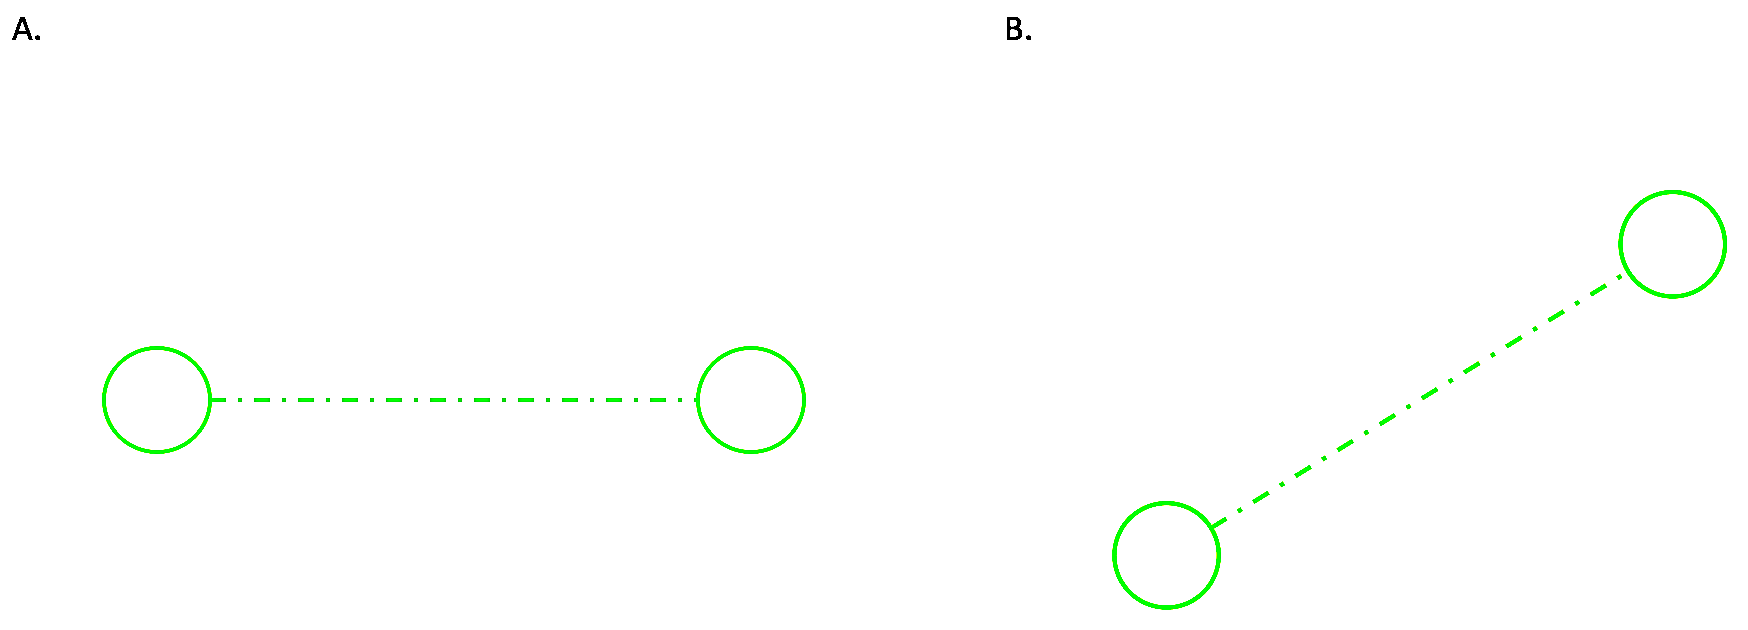
\includegraphics[width=0.8\textwidth]{figs/rotation.png}
	\caption[Caption for LOF]{\emph{A. Two objects (circles) have a relationship of a certain distance $X$.\\ B. A rotated scene showing such relationship. }}
	\label{fig:rotation}
\end{figure}

Therefore, the pattern learning model described here can be very helpful in understanding the relationship between complex scene ("student taking class", "cars stuck in traffic" etc.) while CNN helps the model to recognize individual object in the scene or generate latent representation for individual object.\\

Besides computer vision, the pattern learning model can also be used in natural language processing task, like modeling the relationship (e.g. Q\&A, extension, agreement, etc.) between sentences in a dialogues. Here, we can turn each word/concept to a node (whose label can be the word vector) and the word/concept distance as the edge. Once we turn the conversation exchange into an ARG, we might be able to model different relationship as well.\\

Therefore, combining neural network for individual object and pattern learning for modeling relationship, machines probably can learn complex structure, scenes, conversations and many other things more effectively. I am really excited about what's coming next.

\section{Protein Modeling}

\subsection{Novel Structure Motif in Protein}

While the proof of concept we did in Section \ref{sec:poc} is nice, domain discovery is not a very challenging task. Due to its relatively large size, simple 3D alignment should give you a reasonably good match and you don't really need to model the protein as an ARG.\\

However, if we are able to train the model efficiently with enough data, we might be able to discover 3D structure motifs that have long been overlooked by sequential matching algorithm. If the model can learn such novel motif, it would be of great help for many biologists.

\subsection{Protein as Documents and Amino Acid as Word}

In Section \ref{sssec:a2v}, we treated protein as documents and amino acid as word, which allows us to use model in natural language field to generate representation for amino acid.\\

In the same line, many of the models developed today in the natural language field, especially the kinds dealing with sequential model, might be a great tool for answering question about protein. For instance, we can use a Seq2Seq model to predict structure of protein sequence, or use LSTM model to predict protein chemical property with the protein sequence.


\subsection{Edge for Protein ARG Revisit}

While tuning hyper parameters for the model, we realized that the node compatibility needs to play a more important role(larger $\alpha$) in order to get clear and correct result for graph matching. This makes sense because protein alignment should be driven more by the amino acid compatibility. However, can we give edge here a different representation and a more effective relationship to help with matching/alignment?



% ------------ Bibliography ----------------

% Adds all of the citations to the Paper, regardless of if they are used.
\nocite{*}


% ------------ Appendices ----------------

\chapter{Appendices}



% \input{./appendices/codestructure.tex}

% \input{./appendices/co-cyclesgraphs.tex}

% \input{./appendices/specs.tex}

% \input{./appendices/scorereportsummaries.tex}

% \input{./appendices/randomgraphbaselines.tex}

\end{document}

\end{document}
